% vim: tw=80

\chapter{Theory Predictions for the Triple-Differential Dijet Cross Section}

\section{Discussion of the Diejt Observable}

For a long time, leading-order (LO) and next-to-leading (NLO) predictions
for dijet production processes were the ultimate precision possible. While
describing the shape and the normalization of many cross section distributions
accurately, they are also subject to larger scale uncertainties. 

The goal of this thesis is a publication of a high-precision dijet cross section
measurement to gain a better understanding of the theory of quantum chromodynamics
at high scales accesible at the LHC. Unlike earlier dijet analyses, the observable
choice was optimized to yield the best-possible constraints on the proton PDFs as well
as the strong coupling.

For nearly ten years, theorists have been working on the calculation of next-to
next-to-leading order (NNLO) predictions for dijet cross sections. This  and this
huge project



\section{NLO Prediction}

The NLO cross section of the triple-differential dijet cross section is
calculated using the \NLOJETPP program~\cite{nlojetpp}. To populate the whole
accessible phasespace with sufficient events to get a precise prediction, a huge
number of events is neccessary. Since especially the influence of the PDFs and
the strong coupling constant is interesting to be studied, the calculation would
have to be repeated multiple times with different input parameters. In order to
speed-up this process, \NLOJETPP is interfaced to the \fastNLO
package~\cite{fastnlo}. fastNLO uses sophisticated interpolation tables to store
the matrix element coefficients as a function of the scales, the calculation
order and the fractional proton momentum. The fastNLO tables can now be evaluated with
different PDFs, \as and scales within negligible time. 

\subsection{Scale Choice}

Two different scale choices are investigated in the NLO calculation. 

\subsection{NLO $k$-factors}

To check the influence of the higher-order contributions to the perturbative QCD
prediction, one calculates the differences between the LO prediction and the NLO
prediction, expressed as the ratio $k_\mathrm{NLO}$. 

\begin{equation*}
    k_{\mathrm{NLO}} = \frac{\sigma_{\mathrm{NLO}}}{\sigma_{\mathrm{LO}}}
\end{equation*}

The size of the NLO
correction gives an estimation about the influence of these higher-order
corrections. If they are very small, the LO result already describes the
observable cross section precisely.

\section{Non-Perturbative Corrections}

The NLOJet++ predictions yield a NLO cross section at parton level.  Fixed-order
calculations do not consider any effects from hardronization or multiple parton
interactions, which cannot be described in a these calculations. To be able to
compare the fixed order prediction to the unfolded measurement at particle
level, non-perturbative (NP) corrections are calculated. These corrections are
derived using the MC event generators Pythia8 and Herwig++. The ratio between
the nominal cross section and one withouth hadronization and MPI effects is
taken as the correction~\ref{eq:np_definition} and applied as bin-by-bin corrections to the NLO
prediction.

\begin{equation}
    C^{\mathrm{NP}} = \frac{N^{\mathrm{PS+HAD+MPI}}}{N^{\mathrm{PS}}}
    \label{eq:np_definition}
\end{equation}

For the determination of the non-perturbative corrections, the following
generators and tunes have been used:

\begin{itemize}
    \item Herwig++ with the tune CUETP8M1
    \item Herwig++ with the tune UE-EE-5C
\end{itemize}

\begin{equation}
  f(\ptavg) = A + B \cdot \ptavg^C
  \label{fcn:np_fit}
\end{equation}

The ratio is then fitted using  using a power law function,
see~\ref{fcn:np_fit}.  The envelope of all predictions is used as the
uncertainty on the non-perturbative corrections while the central value of this
envelope is used as the correction factor.  These corrections are of the size of
10 \% to 15 \% at 100 \si{GeV} and get smaller at higher values of \ptavg. Figure
\ref{fig:np_factors} shows the resulting correction factors and the
corresponding uncertainty.

\begin{figure}[htbp]
    \centering
    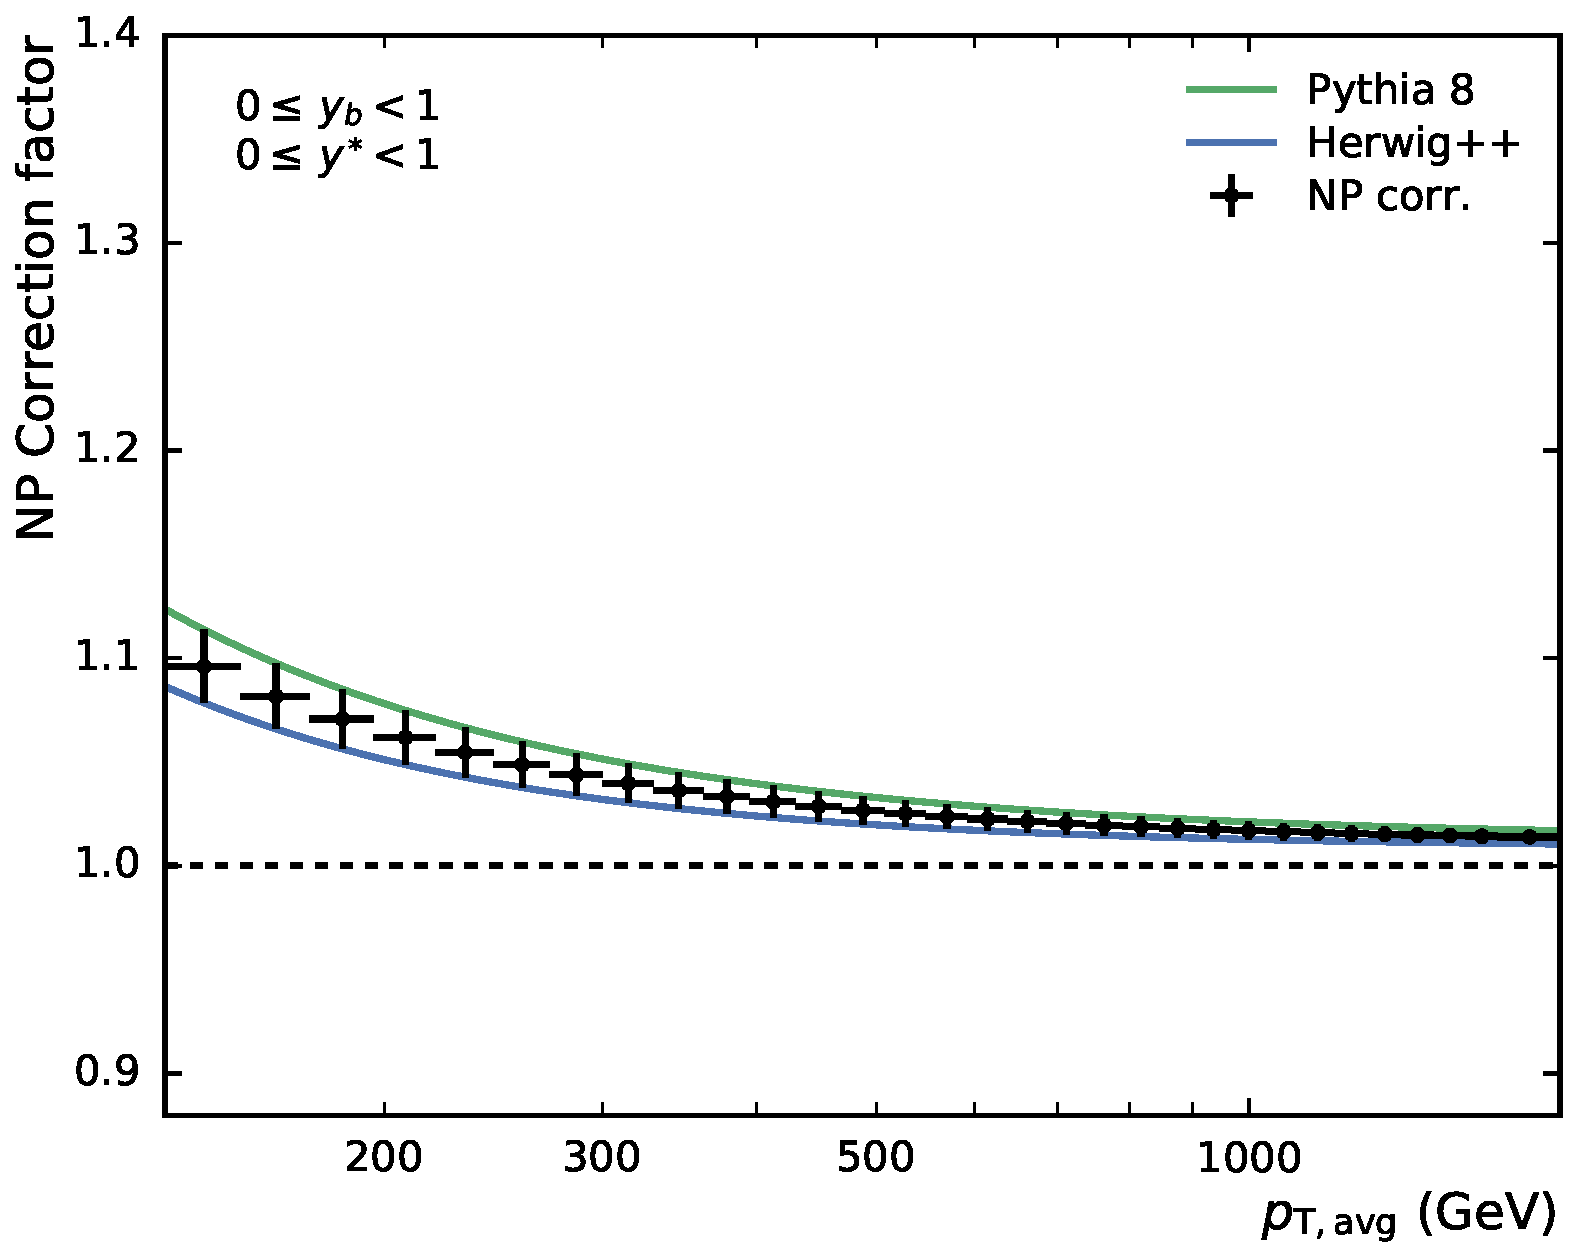
\includegraphics[width=0.45\textwidth]{figures/theory/np_factors_calc_yb0ys0.pdf}\hfill
    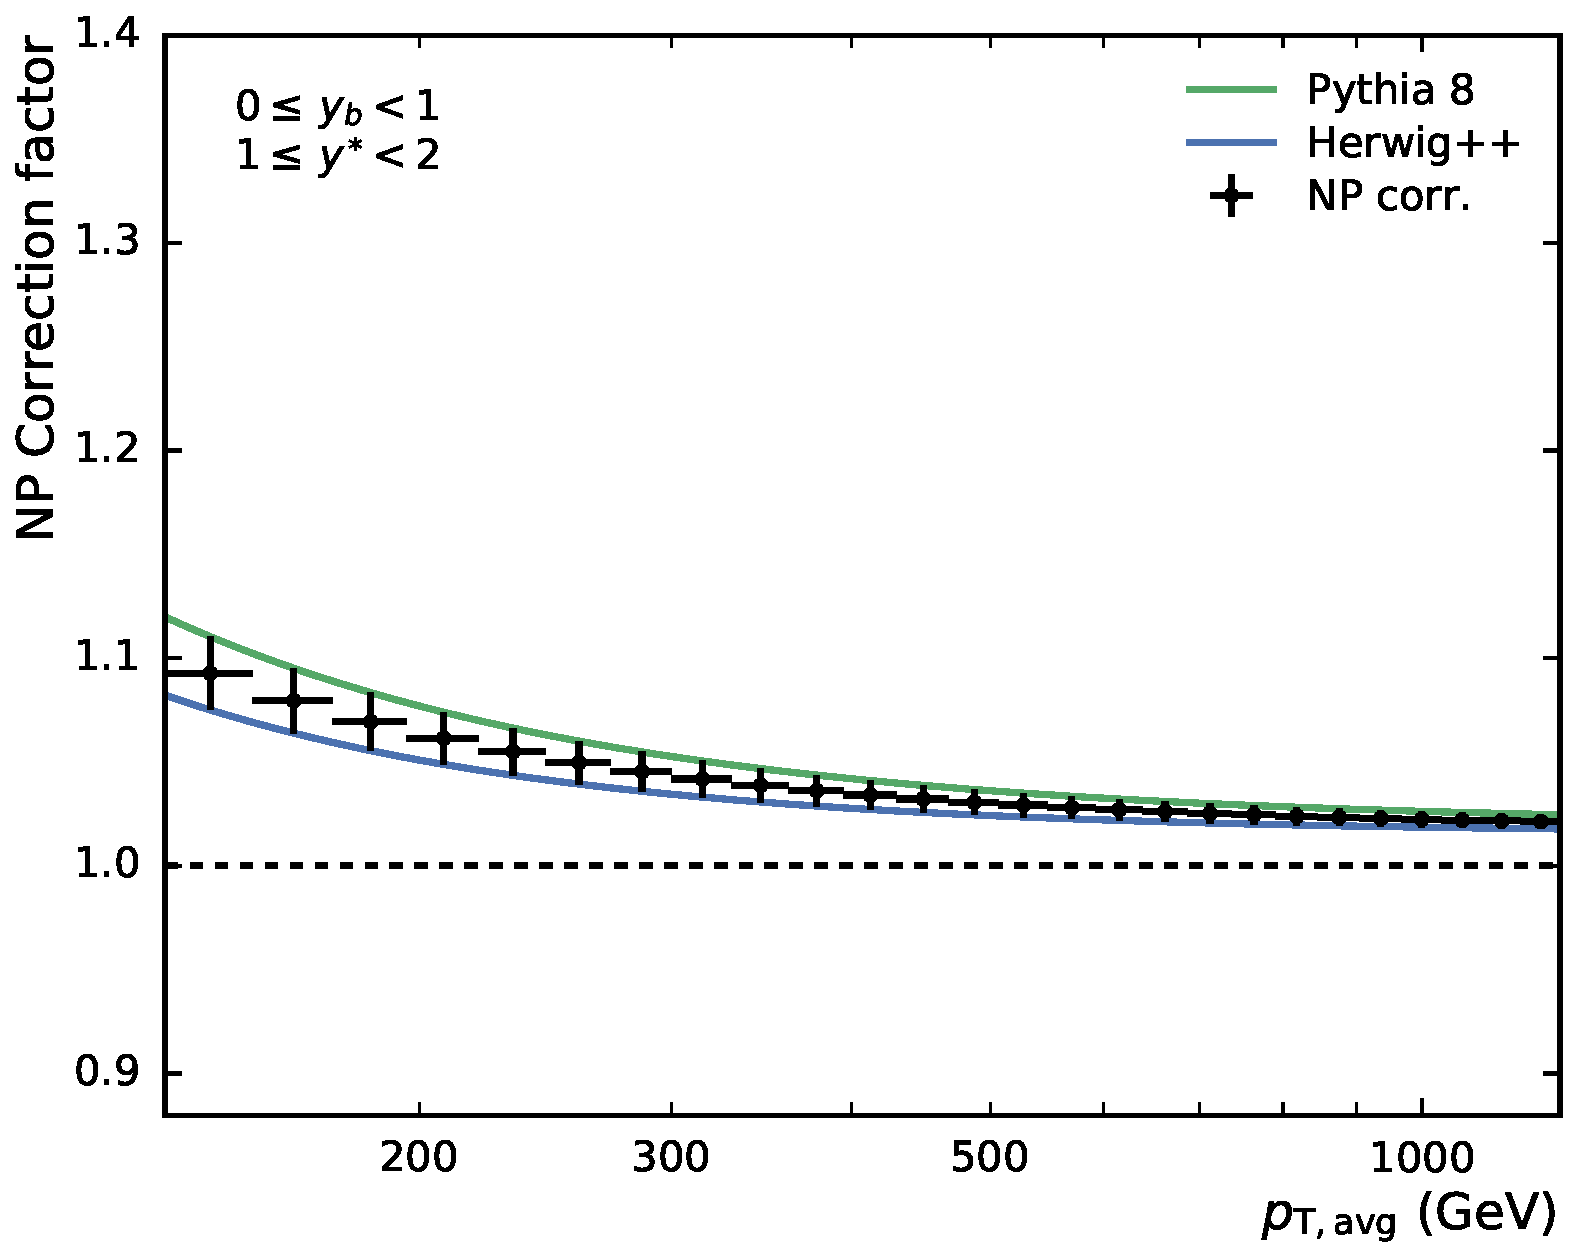
\includegraphics[width=0.45\textwidth]{figures/theory/np_factors_calc_yb0ys1.pdf}
    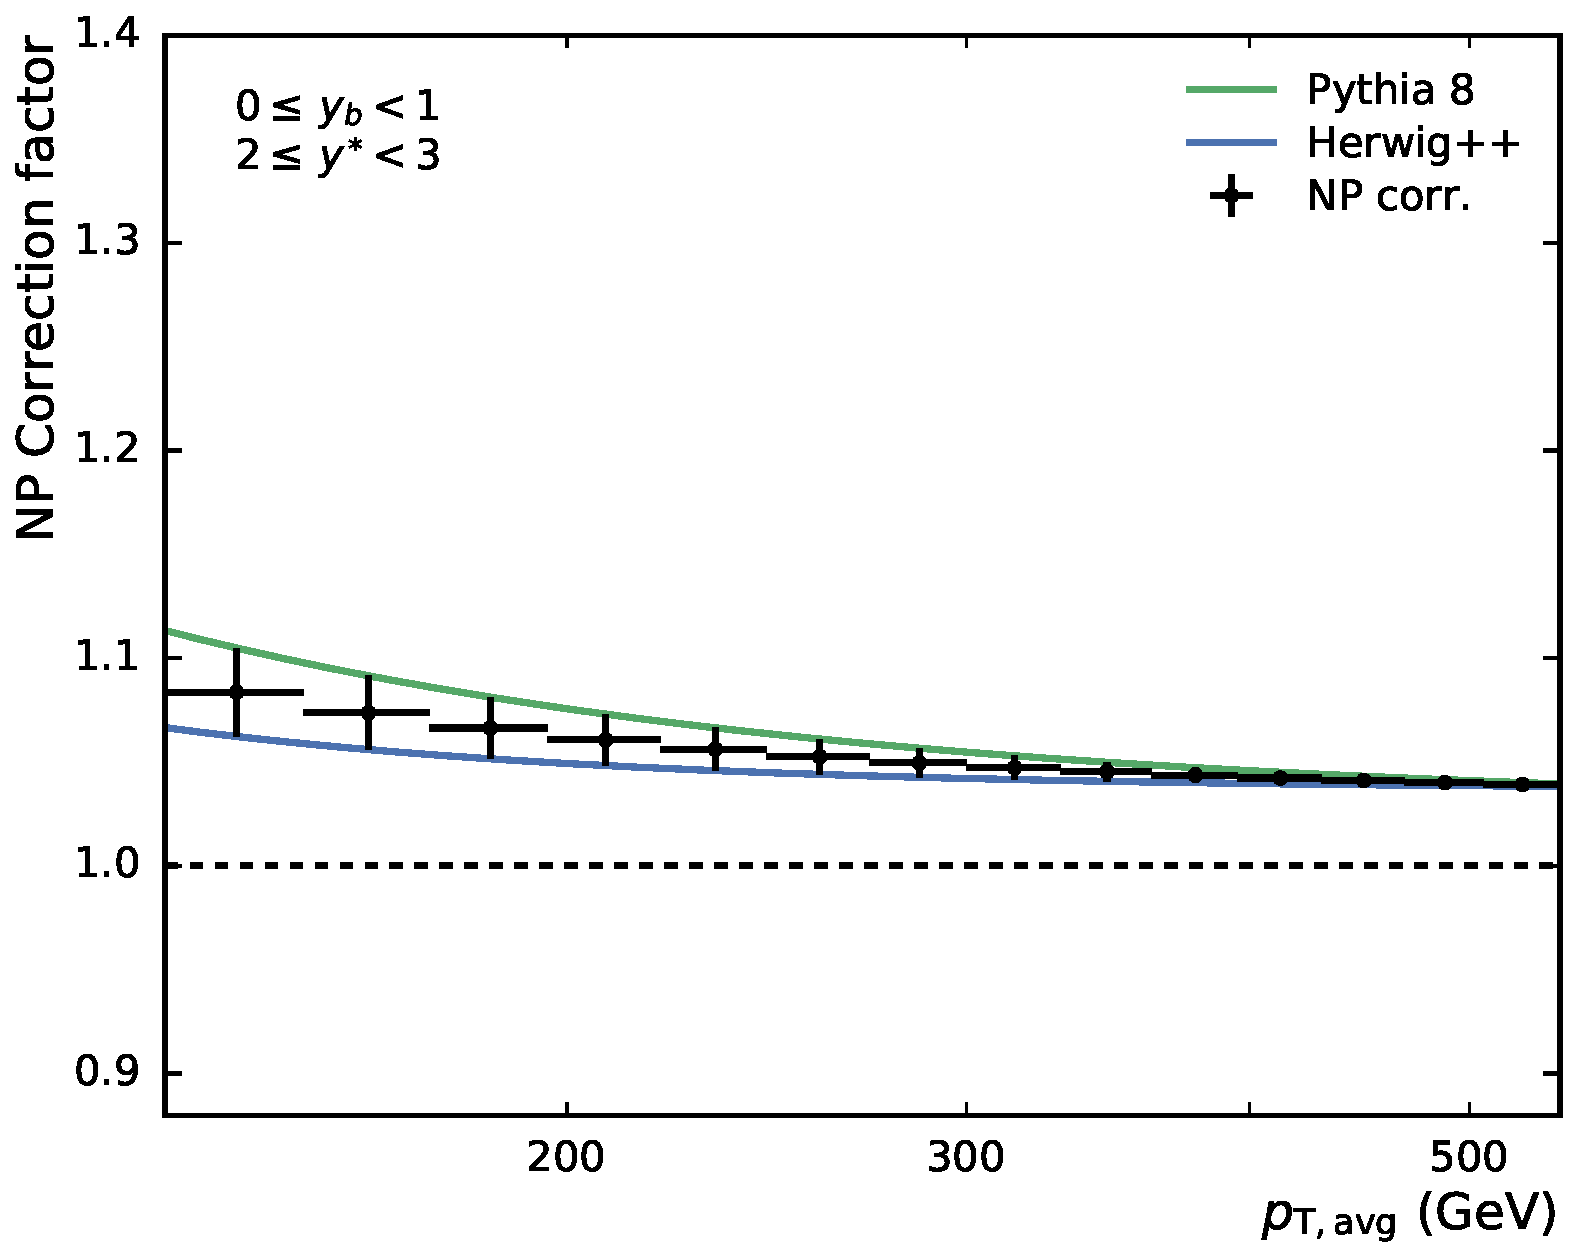
\includegraphics[width=0.45\textwidth]{figures/theory/np_factors_calc_yb0ys2.pdf}\hfill
    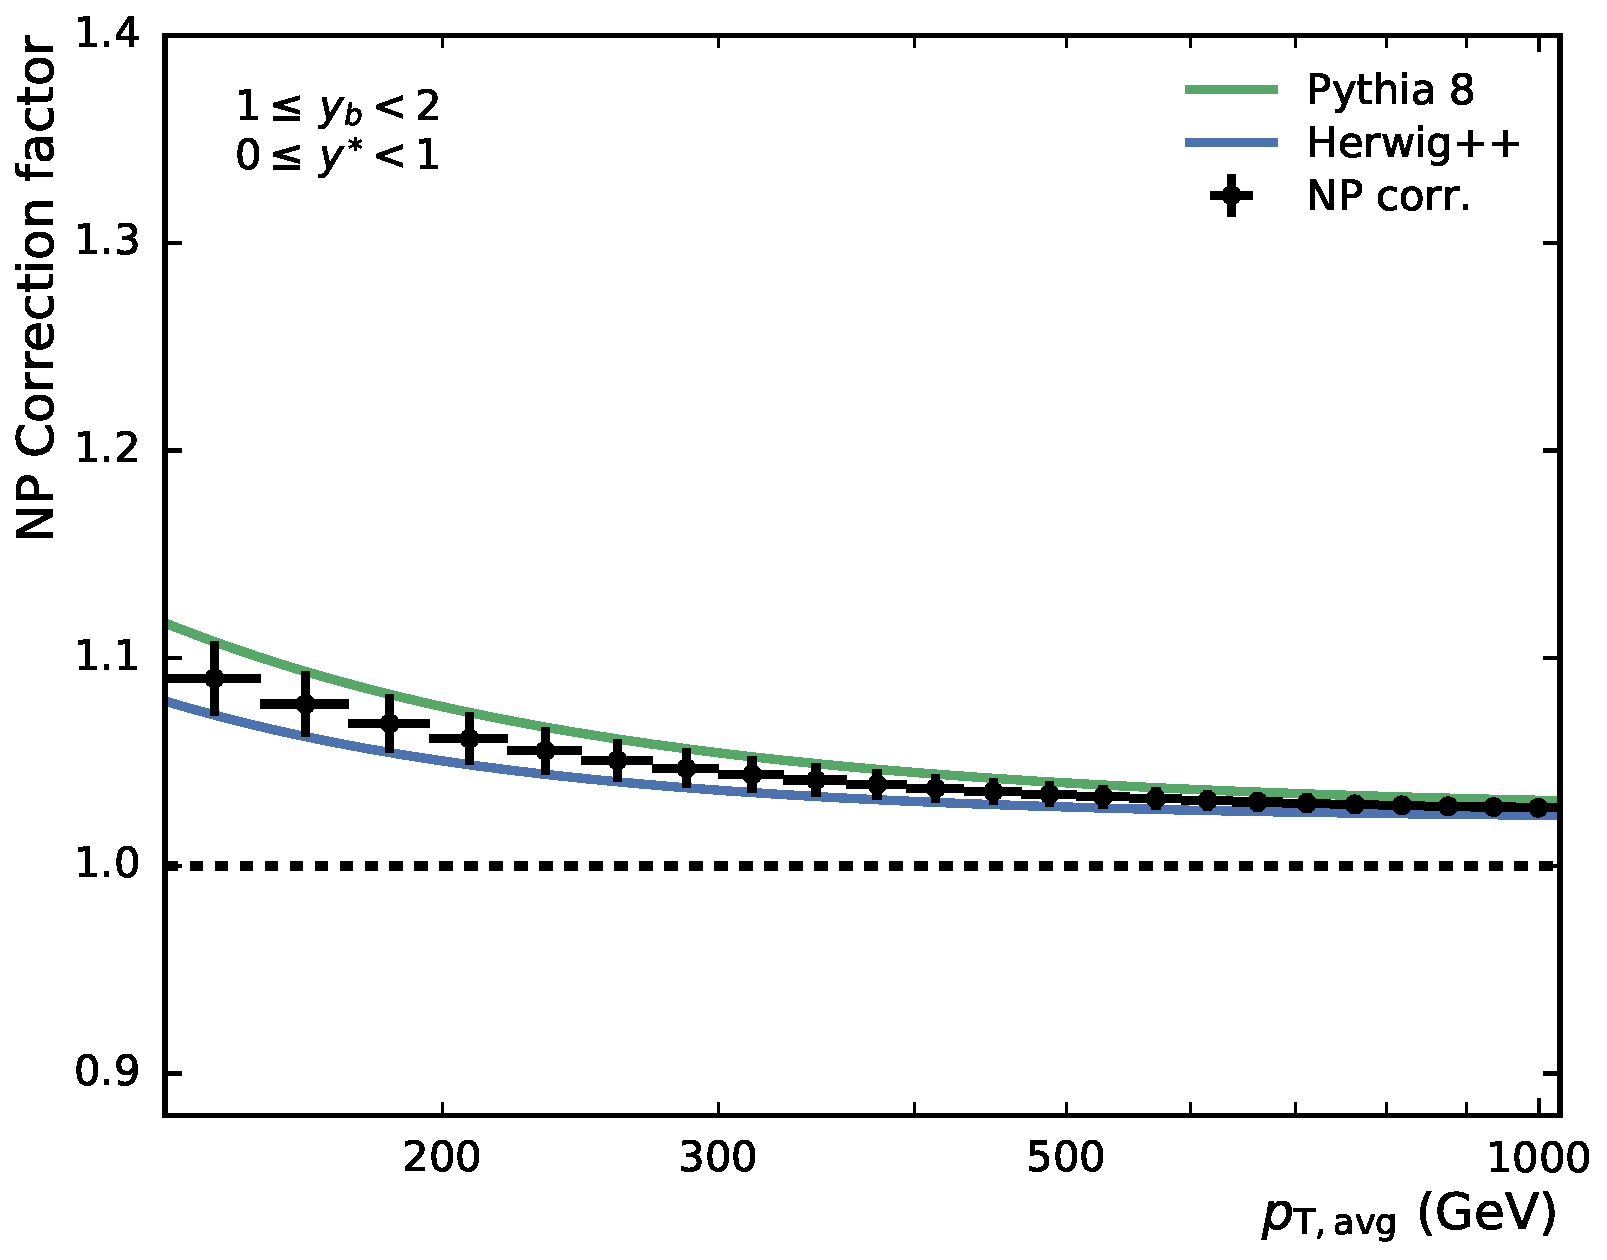
\includegraphics[width=0.45\textwidth]{figures/theory/np_factors_calc_yb1ys0.pdf}
    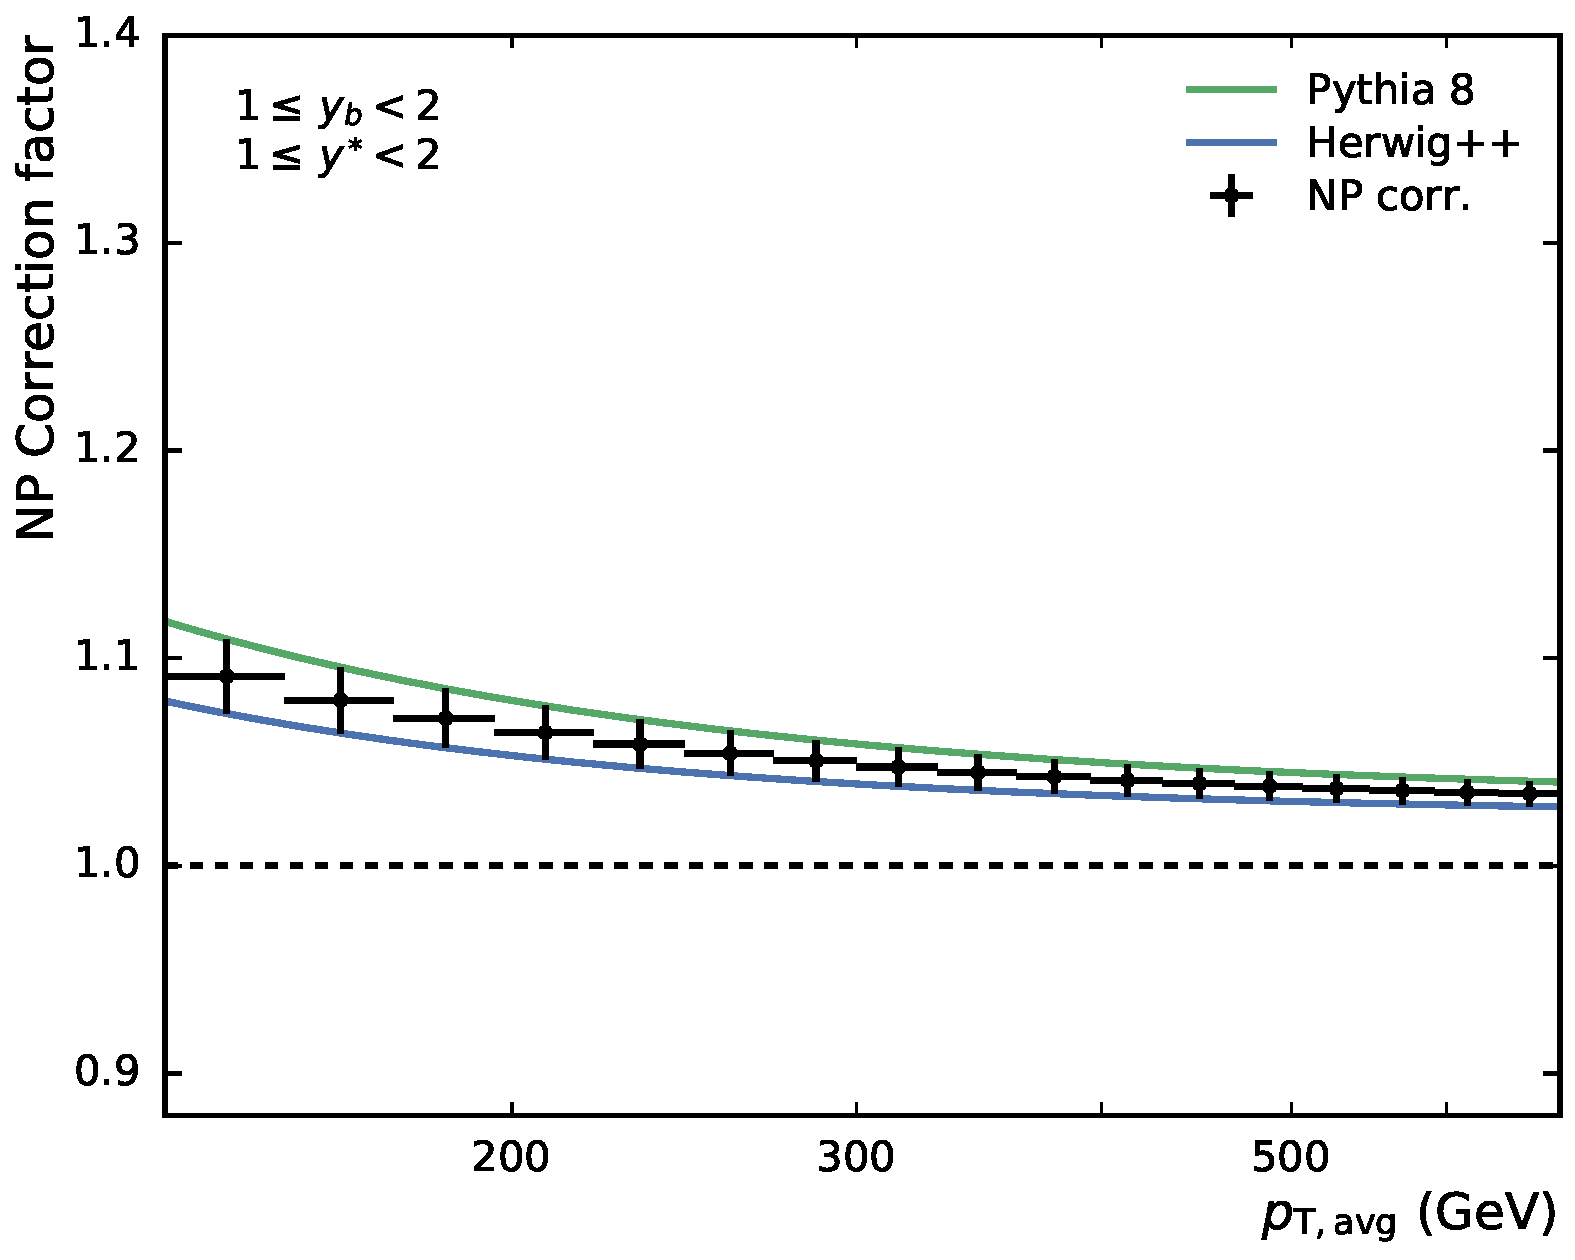
\includegraphics[width=0.45\textwidth]{figures/theory/np_factors_calc_yb1ys1.pdf}\hfill
    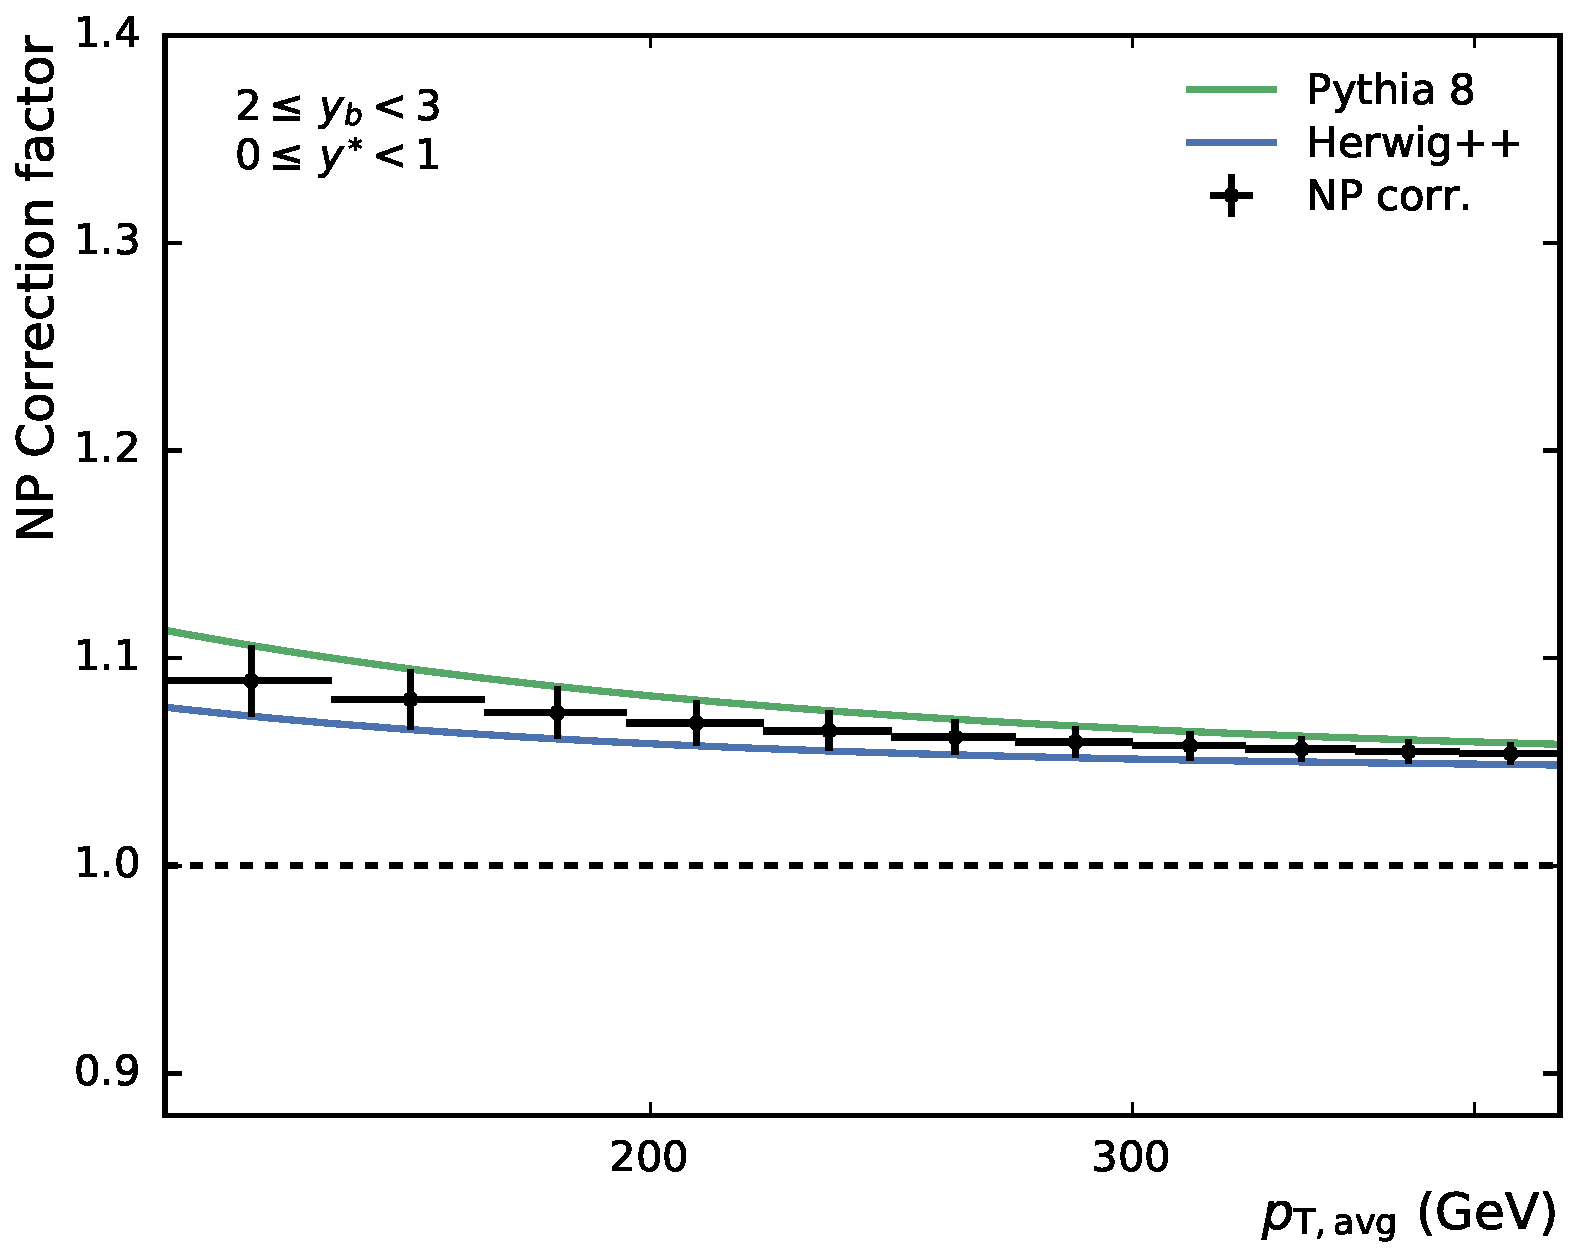
\includegraphics[width=0.45\textwidth]{figures/theory/np_factors_calc_yb2ys0.pdf}
    \caption{The non-perturbative correction is derived using a MC event
    generator by calculating the diferences by including hadronization and MPI
    in the simulation. The green line shows the correction of Pythia 8, the blue
    line the correction of Herwig++. The average of both gives the central
correction and the envelope the uncertainty on the correction.}
    \label{fig:np_factors}
\end{figure}


\section{Theory Uncertainties}

Four sources of uncertainty limit the precision of the NLO theory preidction.
Thi section describes the derivation of the scale, PDF, \as and NP
uncertainties. Depending on the phasespace region the PDF or scale uncertainty
is the dominant source of uncertainty. The fastNLO table is
constructed from statistically independent calculations which are merged to
yield a high number of events. By estimating the uncertainty on the arithmetic
mean of all tables, the statistical uncertainty is found to be smaller than 0.5
\% in all bins, in most of the bins even smaller than 0.1 \%. Therefore the
statistical uncertainty was neglected in all further comparisons.

\subsection{Scale uncertainties}

Within the perturbative cross section calculations, one has to choose a
factorisation and renormalisation scale. The influence of these scales vanishes
when the calculation is performed for all orders of the perturbative series.
However since we truncate the series at NLO, a scale dependence on our result is
introduced. 

While the choice of the scale $\mu$ is per se arbitrary, it should reflect the
energy scale of the interaction. 

There is common approach in estimating the influence of the scale on the cross
section. The cross section calculation is performed using different scale
choices and the differences to the central scale choice is translated into an
uncertainty, called scale uncertainty. The variations are applied as relative
factors to the central choice in the following six combinations: $(\mur, \muf) =
(\sfrac{1}{2}, \sfrac{1}{2}), (\sfrac{1}{2}, 1), (1, \sfrac{1}{2}), (1, 2), (2,
1)$ and $(2, 2)$. The uncertainty is the envelope of the maximum deviation in
the upwards and downwards direction.  Figure~\ref{fig:theo_uncertainties} shows
the relative size of the scale uncertainty for each of the measurement bins.

\subsection{PDF uncertainties}

The dependence of the cross section calculation on the proton structure is
expressed in terms of parton distribution functions, which are derived from a
fit to data from different experiments. There are different sources of
uncertainty introduced when deriving the PDFs. These include the choice and the
functional form of the parametrization, the chosen theory model and input
parameters like the strong coupling or the quark masses as well as the data
uncertainties which are propagated onto the PDFs.

There derivation of PDF uncertainties follows prescriptions of each individual
PDF set. The NNPDF PDF sets use Monte-Carlo pseudoexperiments, in which the PDF
fit is performed using data smeared within their uncertainties taking into
account the correlations. These so-called replicas are then averaged to give the
central result and the spread of the replicas determines the uncertainty. The
PDF uncertainty of a quantity $X$ which can be a cross section calculation or
even the PDF itself is expressed as

\begin{equation*}
    \Delta X = \sqrt{\frac{1}{N-1} \sum_{i=1}^N \left( X_{i} - X_{\mathrm{central}} , 0 \right)^2}
\end{equation*}

The CT14 and MMHT PDF sets both employ the eigenvector method to encode the
uncertainties. A transformation from the parameter basis to the eigenvector
basis is done to yield mutually uncorrelated eigenvectors. By varying the
eigenvectors upwards and downwards, a set of eigenvector pairs is generated which can used to
determine the asymmetric uncertainty $X_+$ and $X_-$ of a quantity..

\begin{equation*}
\begin{aligned}
\Delta X^+ &= \sqrt{\sum_i^{N_{\mathrm{EV}}} \left[ \max(X_i^+ -X_0, X_i^- - X_0, 0)\right]^2}\\
\Delta X^- &= \sqrt{\sum_i^{N_{\mathrm{EV}}} \left[ \min(X_i^+ -X_0, X_i^- - X_0,0)\right]^2}
\end{aligned}
\end{equation*}

The symmetric uncertainty is given by half the difference of the upwards and
downwards variation.

\begin{equation*}
    \Delta X = \sqrt{\sum_i^{N_{\mathrm{EV}}} \left[ \frac{\left( X_i^+ -
    X_i^-\right)}{2} \right]^2}
\end{equation*}

The CT14 PDF uncertainties describe a 90\% confidence interval while the MMHT
and NNPDF PDF uncertainties represent a 68\% confidence interval. The CT14
uncertainties are scaled to 68CL using $s = \sqrt{2} \erf^{-1}(0.9) = 1.645$.
Figure~\ref{fig:pdf_uncertainties} shows the fractional PDF uncertainty for
these three PDF sets. The PDF uncertainty in the bins with a small \ystar and a
small \yboost value is comparably small. This is due to the fact that mostly
events with two jets which are balanced in rapidity contribute. The PDF
uncertainty in the bin with high \ystar value and a low \yboost value, in which
two forward jets which are back-to-back in rapidity is similar and not sizeable.
The most interesting region is the one with a high \yboost value. There the
rapidity of both jets has the same sign and is large. To achieve this high boost, one
must access the high-$x$ region of one proton, which is not well known and is
afflicted with large PDF uncertainties. Especially the NNPDF PDF set has a large
uncertainty in this region. This is caused by the very flexible parametrization
of the NNPDF PDF set which results in large PDF uncertainty in phase space
regions not covered by data.

\begin{figure}[htbp]
    \centering
    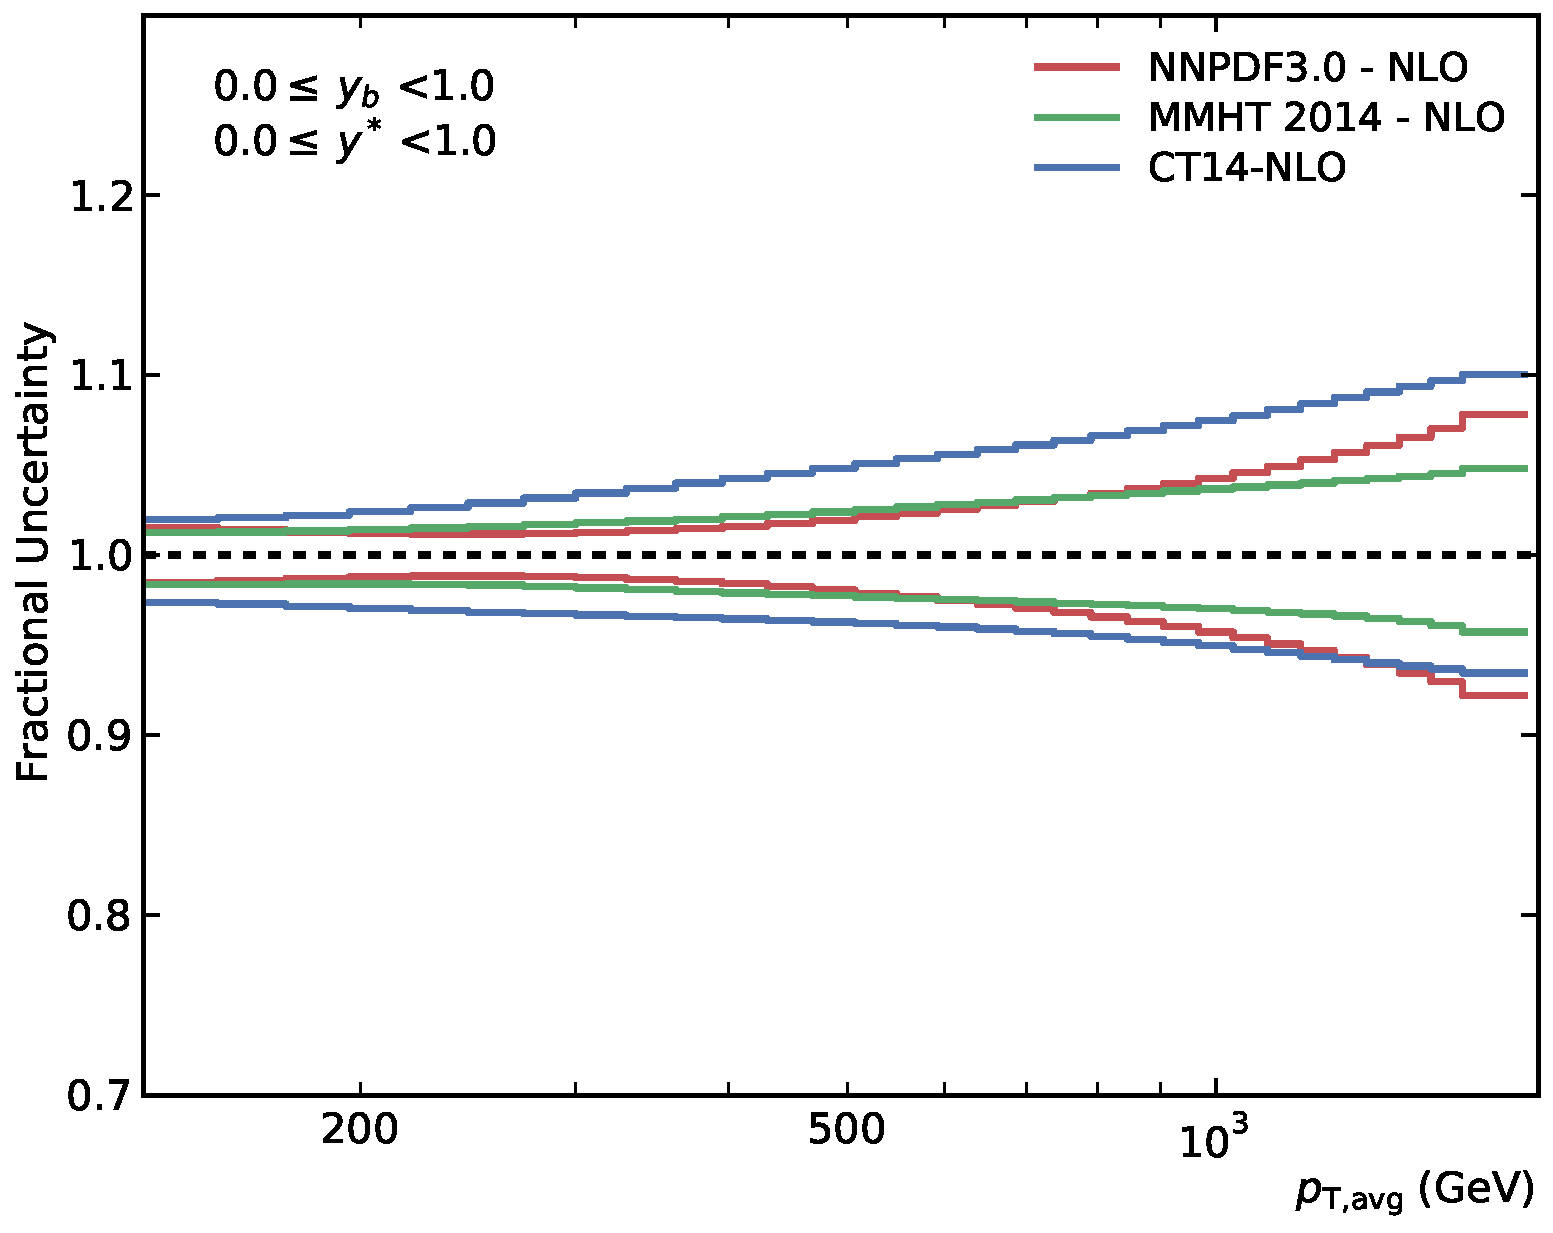
\includegraphics[width=0.45\textwidth]{figures/theory/pdf_unc_comparison_yb0ys0.pdf}\hfill
    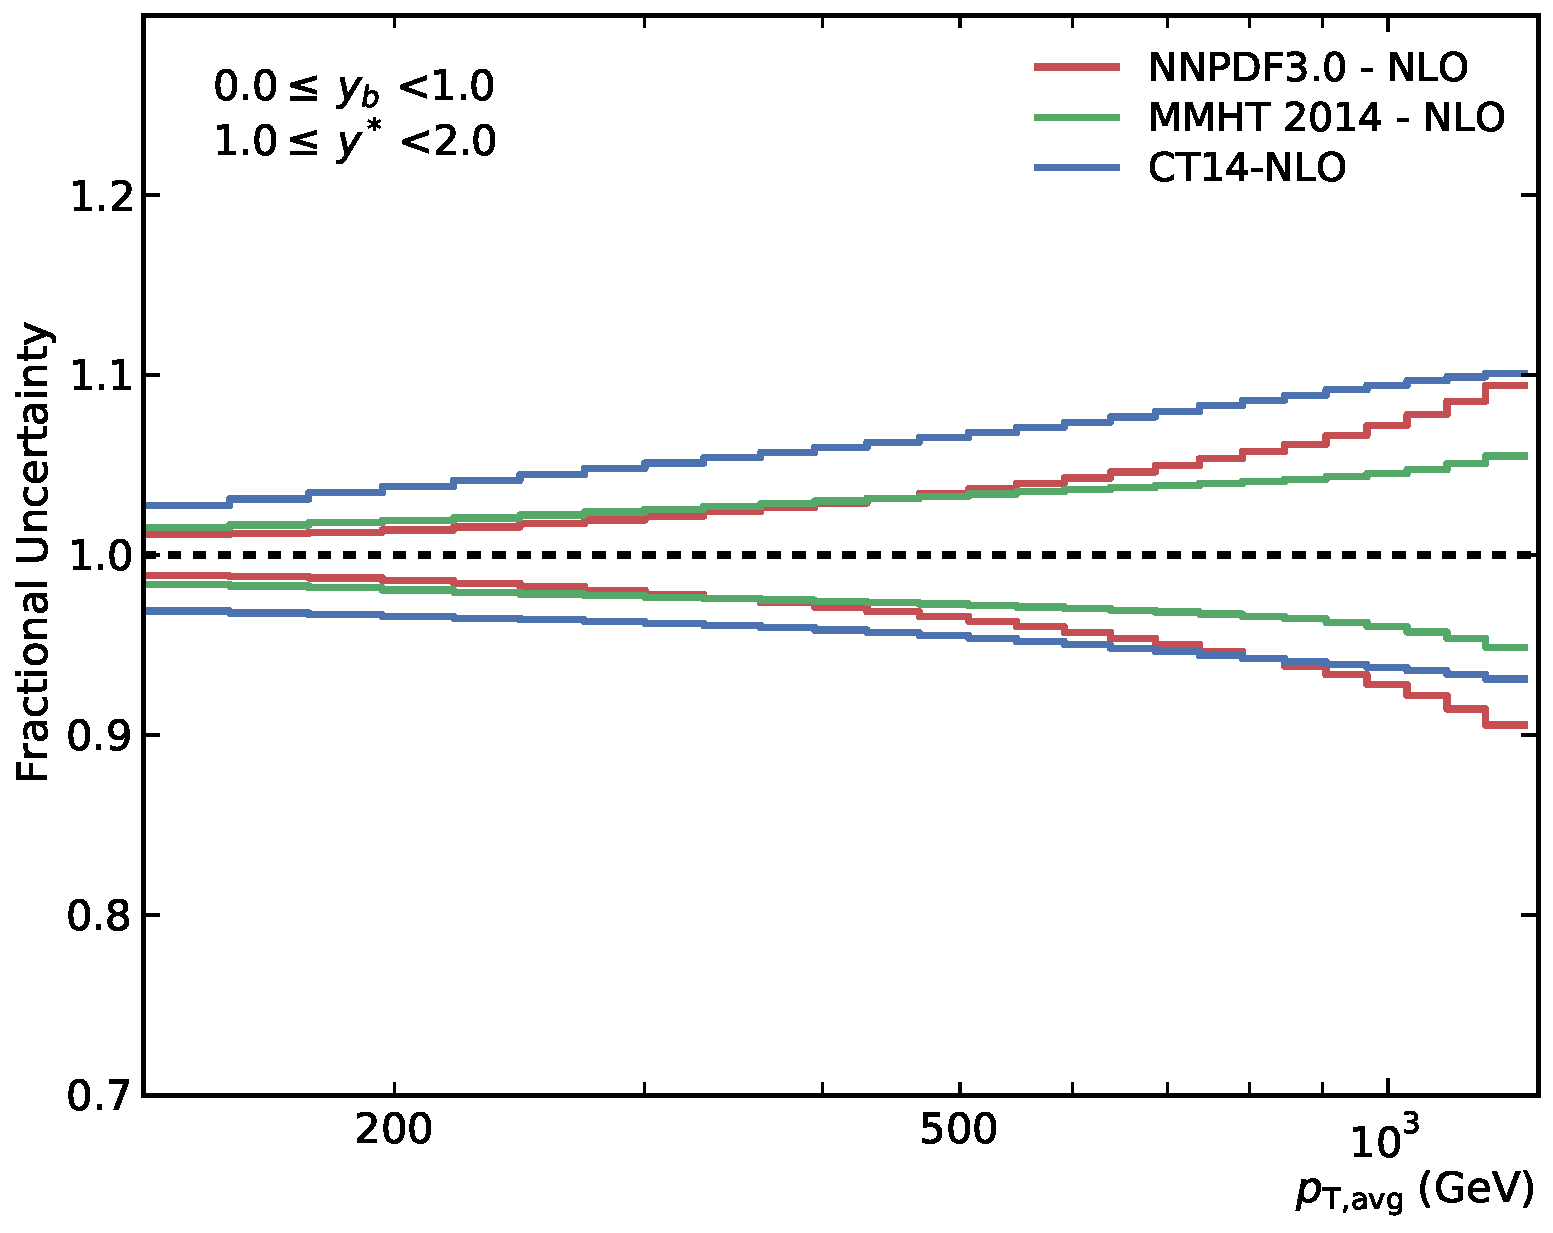
\includegraphics[width=0.45\textwidth]{figures/theory/pdf_unc_comparison_yb0ys1.pdf}
    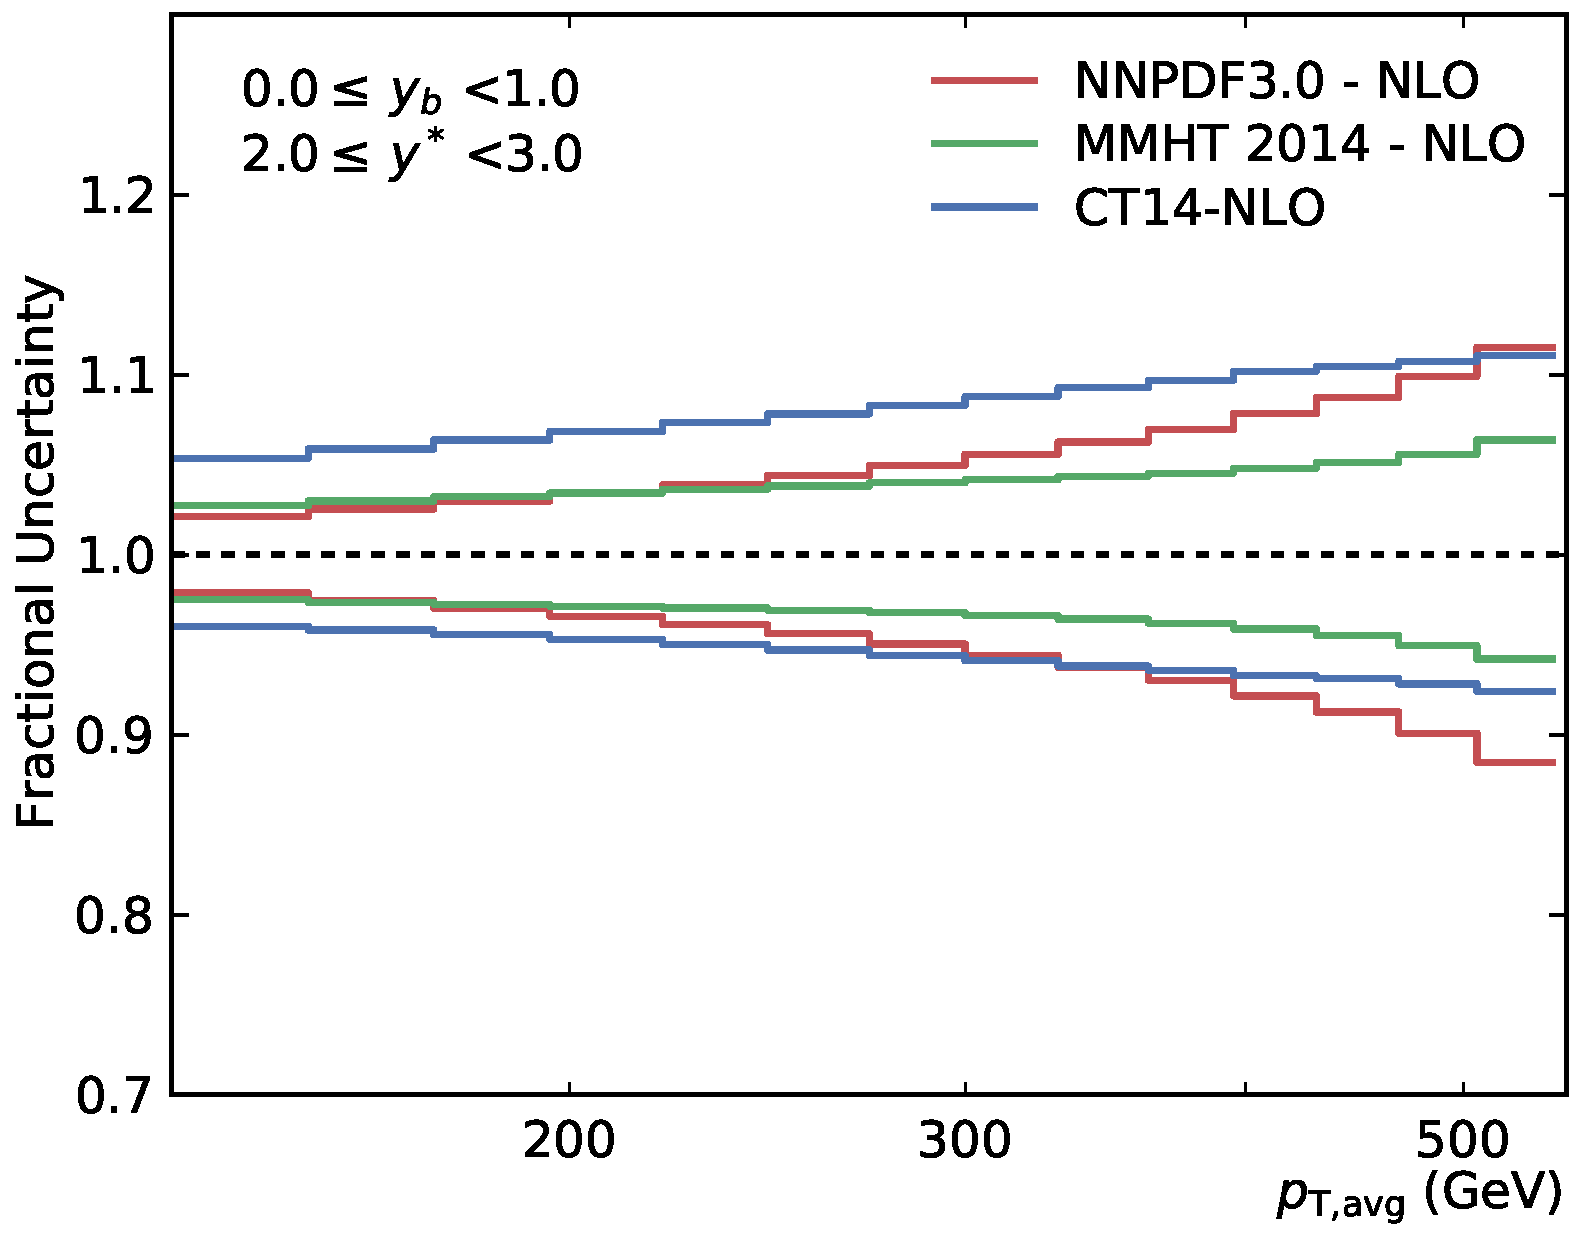
\includegraphics[width=0.45\textwidth]{figures/theory/pdf_unc_comparison_yb0ys2.pdf}\hfill
    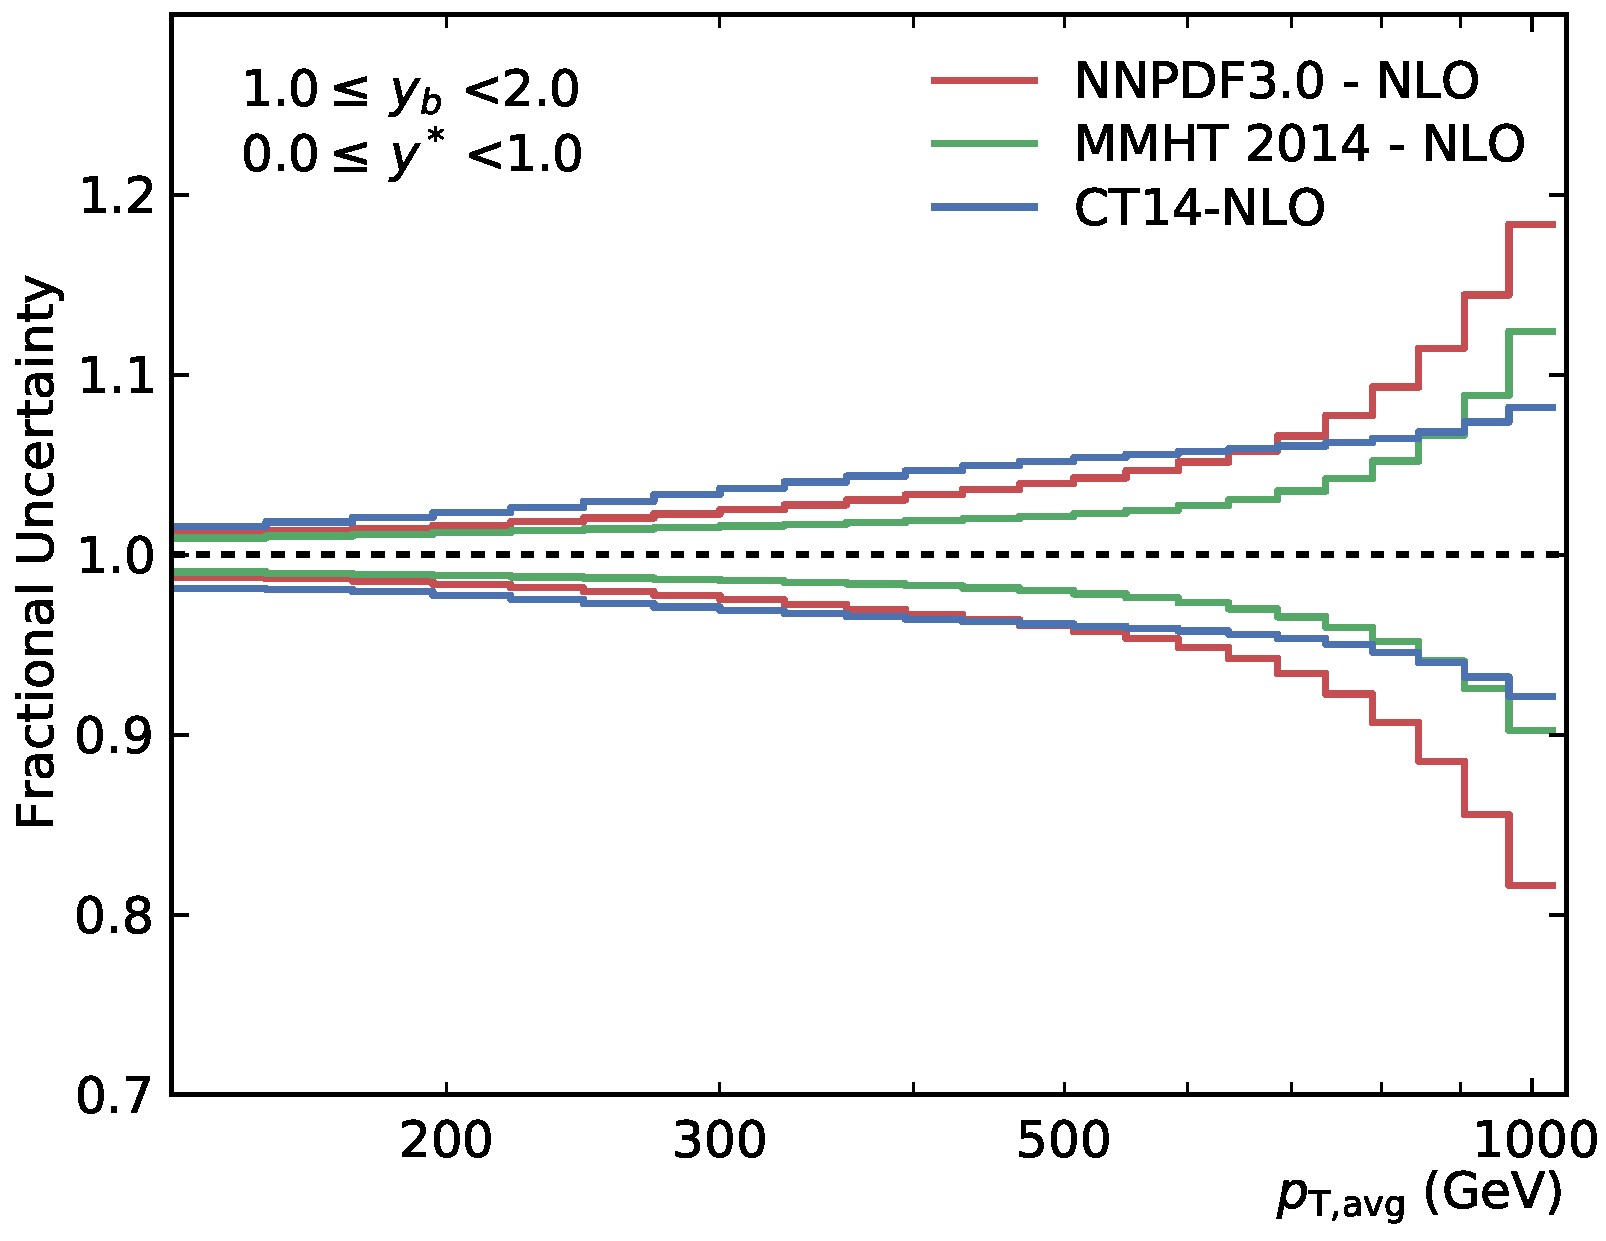
\includegraphics[width=0.45\textwidth]{figures/theory/pdf_unc_comparison_yb1ys0.pdf}
    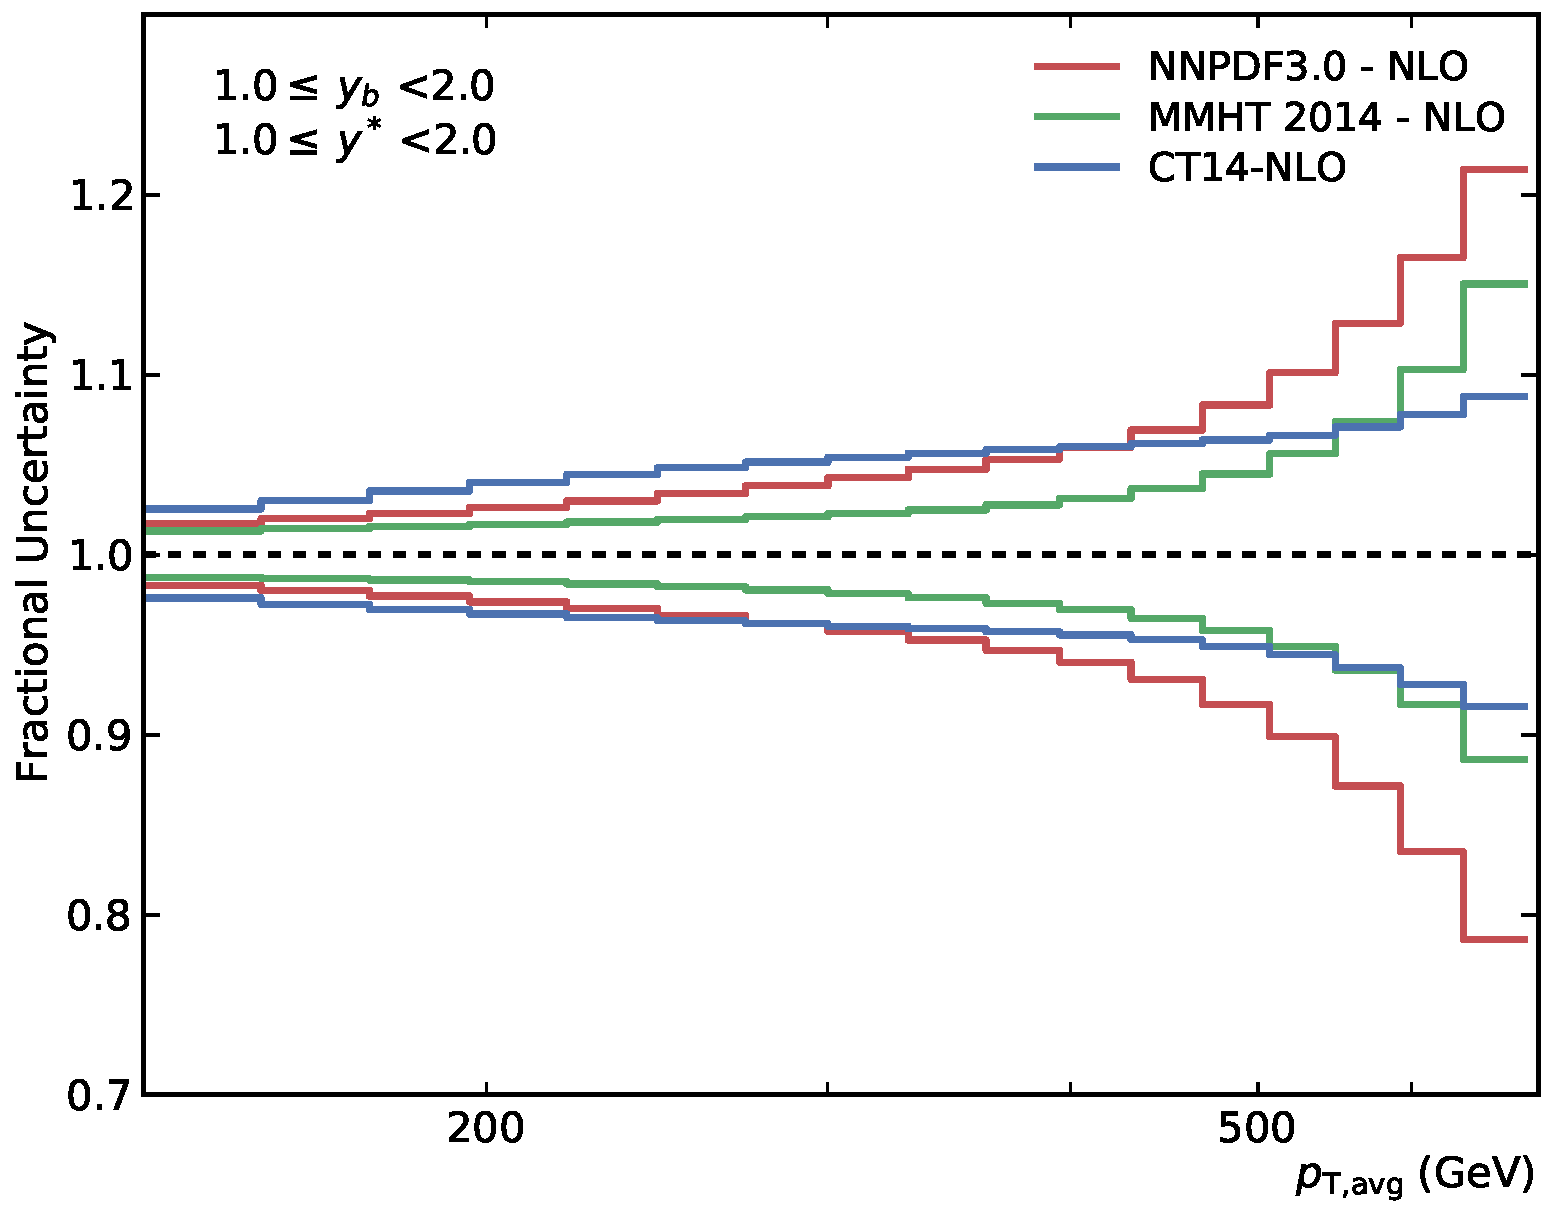
\includegraphics[width=0.45\textwidth]{figures/theory/pdf_unc_comparison_yb1ys1.pdf}\hfill
    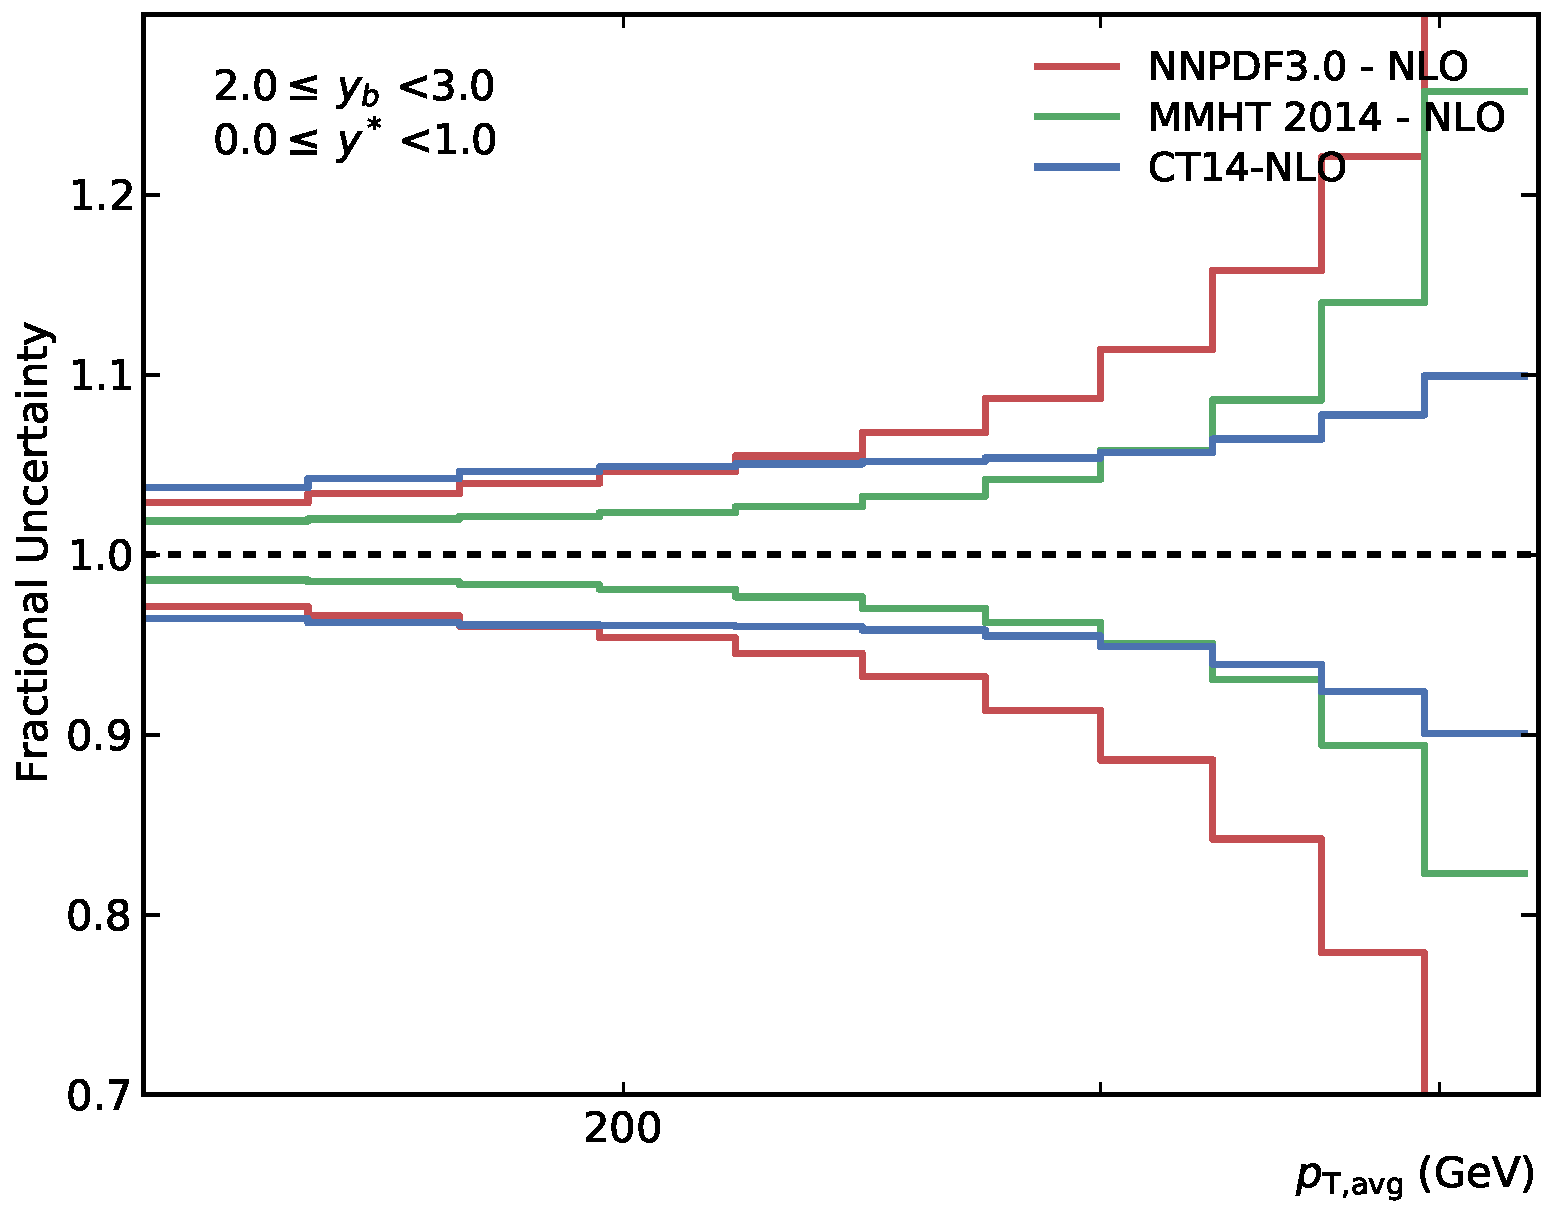
\includegraphics[width=0.45\textwidth]{figures/theory/pdf_unc_comparison_yb2ys0.pdf}
    \caption{The relative PDF uncertainty calculated using the three PDF sets
    NNDFP 3.0, CT14 and MMHT 2014. The uncertainty represents a 68\% confidence
    interval. The PDF uncertainty is sizeable especially in the forward region in
    which both jets have the same sign and high fractional proton momenta are
    accessed. }
    \label{fig:pdf_uncertainties}
\end{figure}

\begin{figure}[htbp]
    \centering
    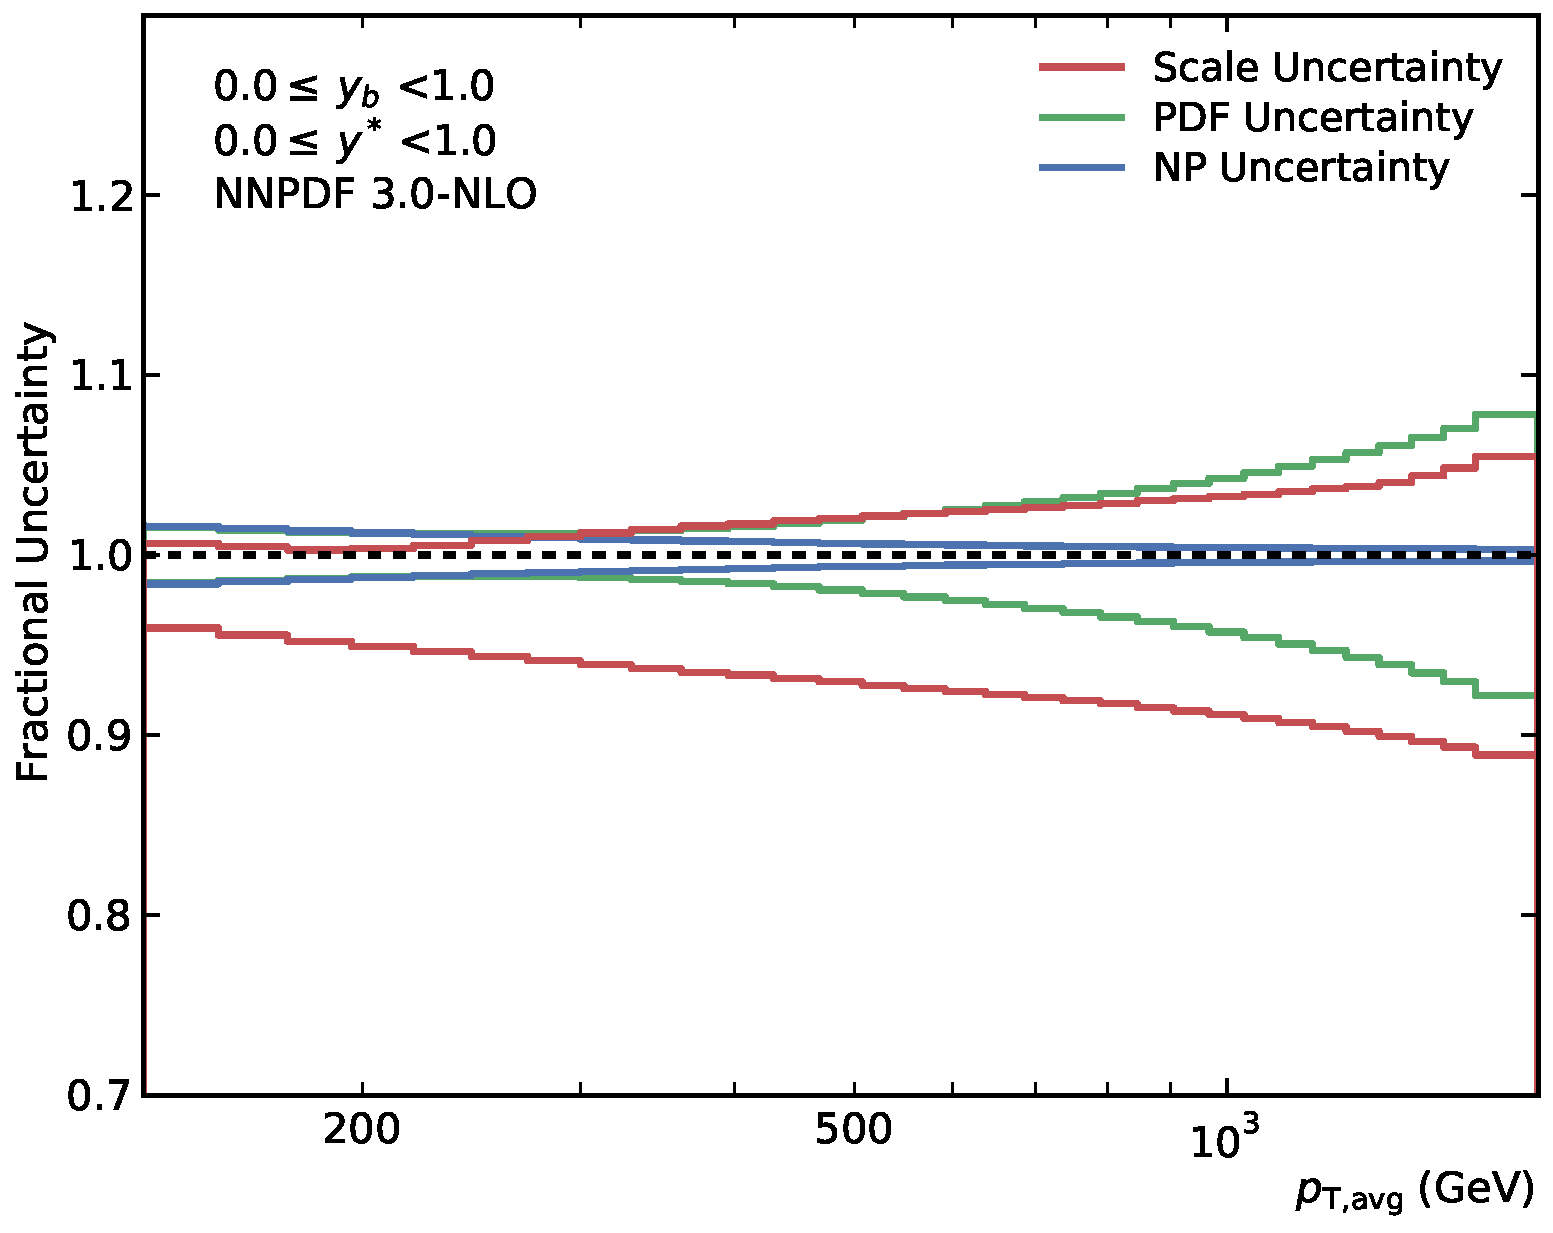
\includegraphics[width=0.45\textwidth]{figures/theory/theo_unc_yb0ys0.pdf}\hfill
    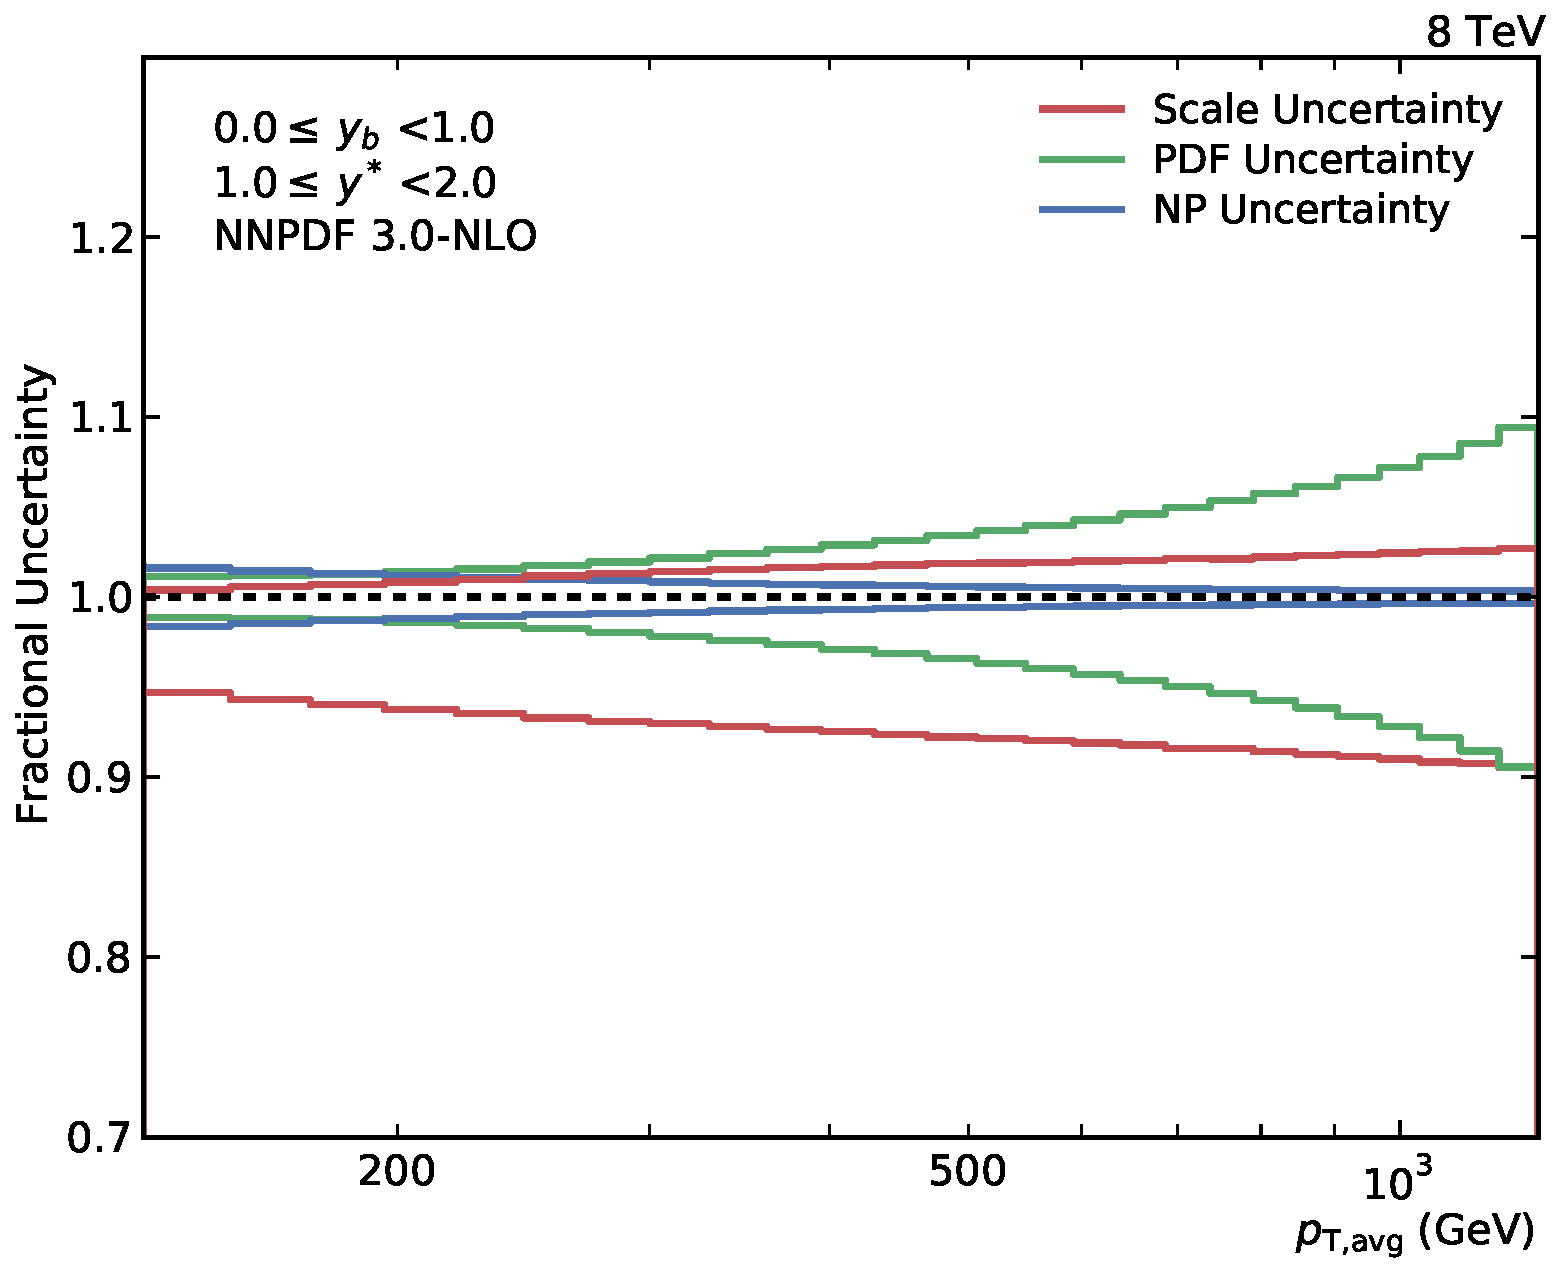
\includegraphics[width=0.45\textwidth]{figures/theory/theo_unc_yb0ys1.pdf}
    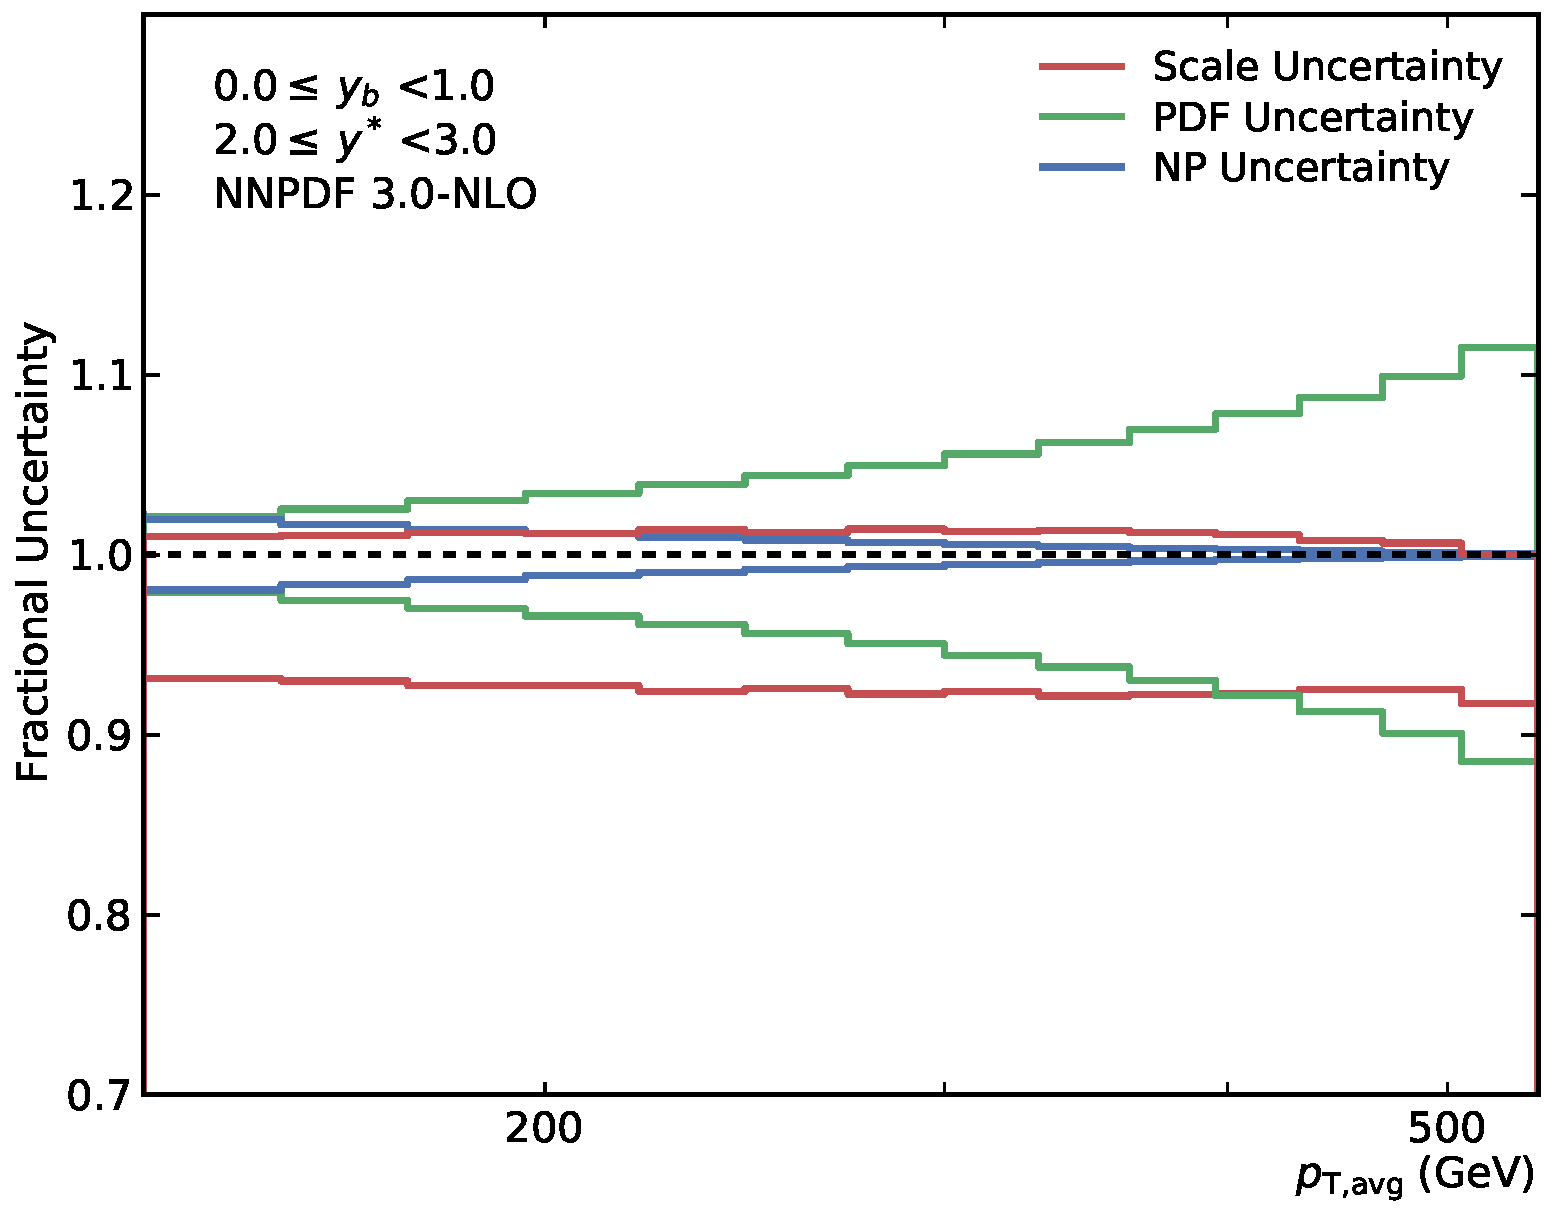
\includegraphics[width=0.45\textwidth]{figures/theory/theo_unc_yb0ys2.pdf}\hfill
    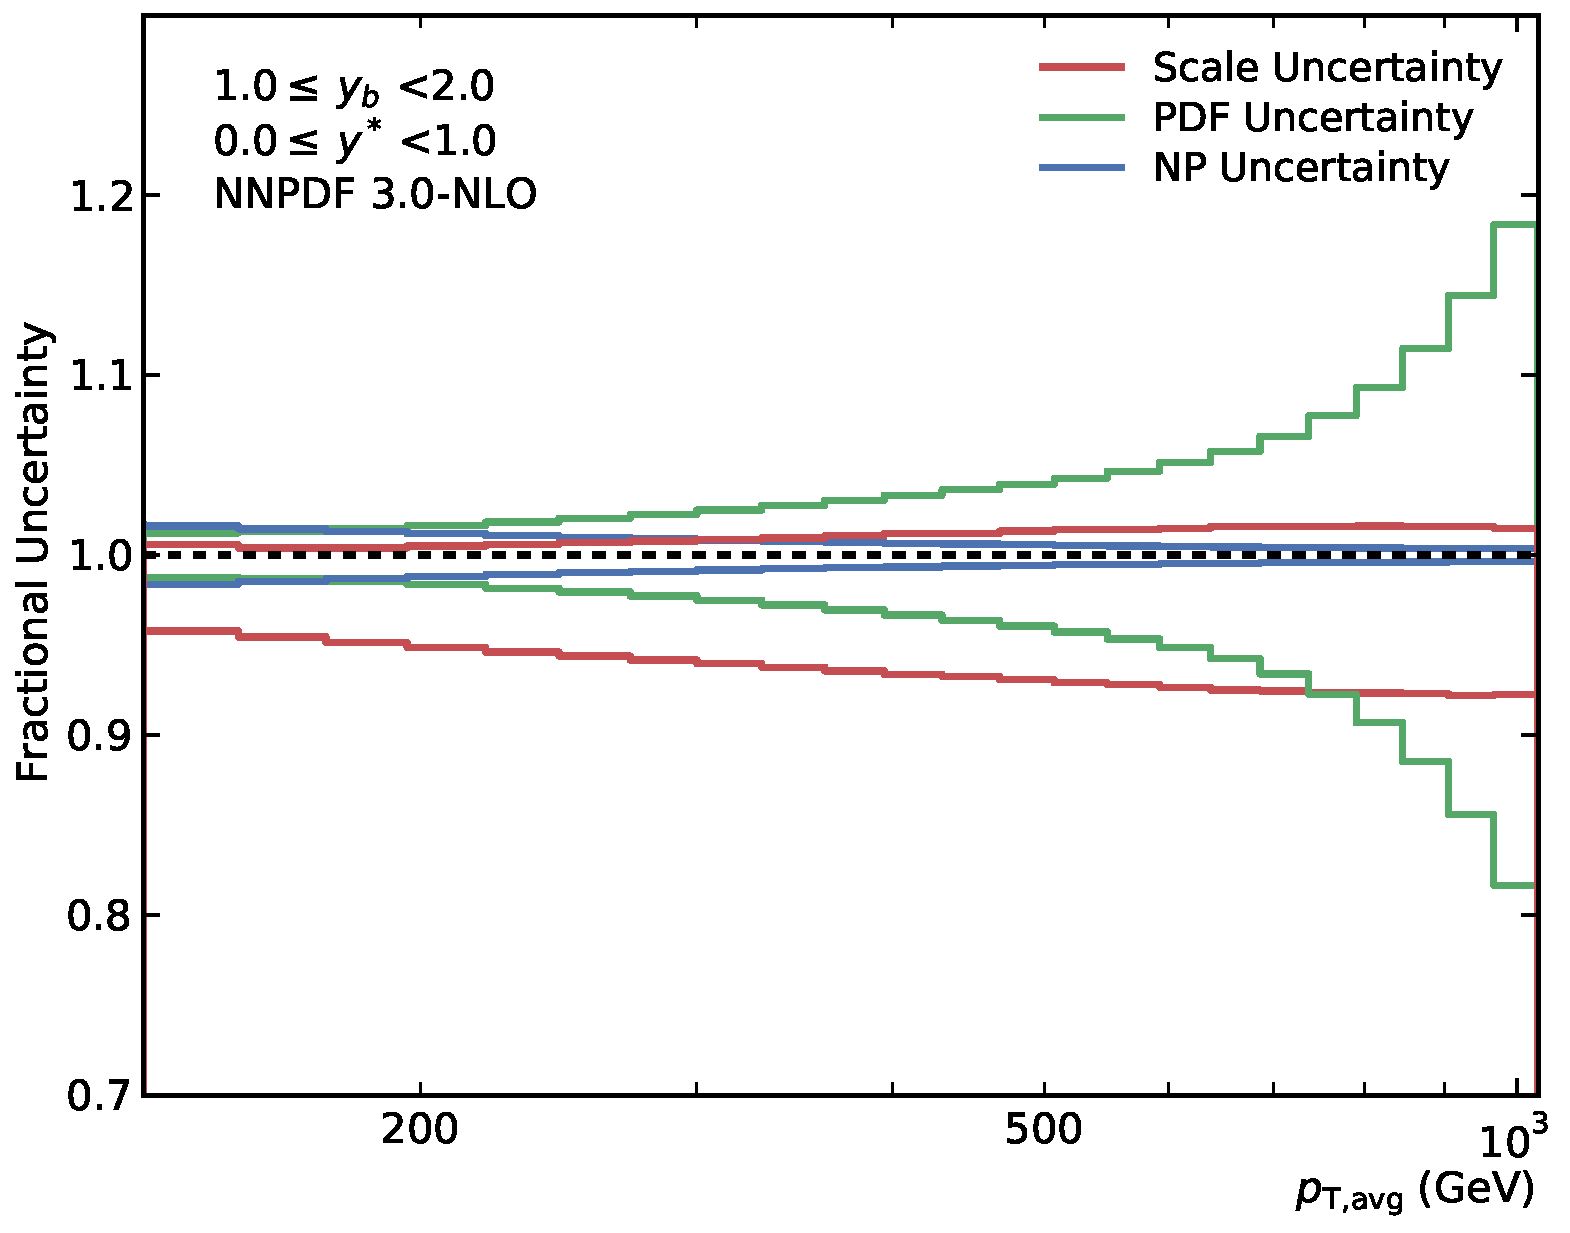
\includegraphics[width=0.45\textwidth]{figures/theory/theo_unc_yb1ys0.pdf}
    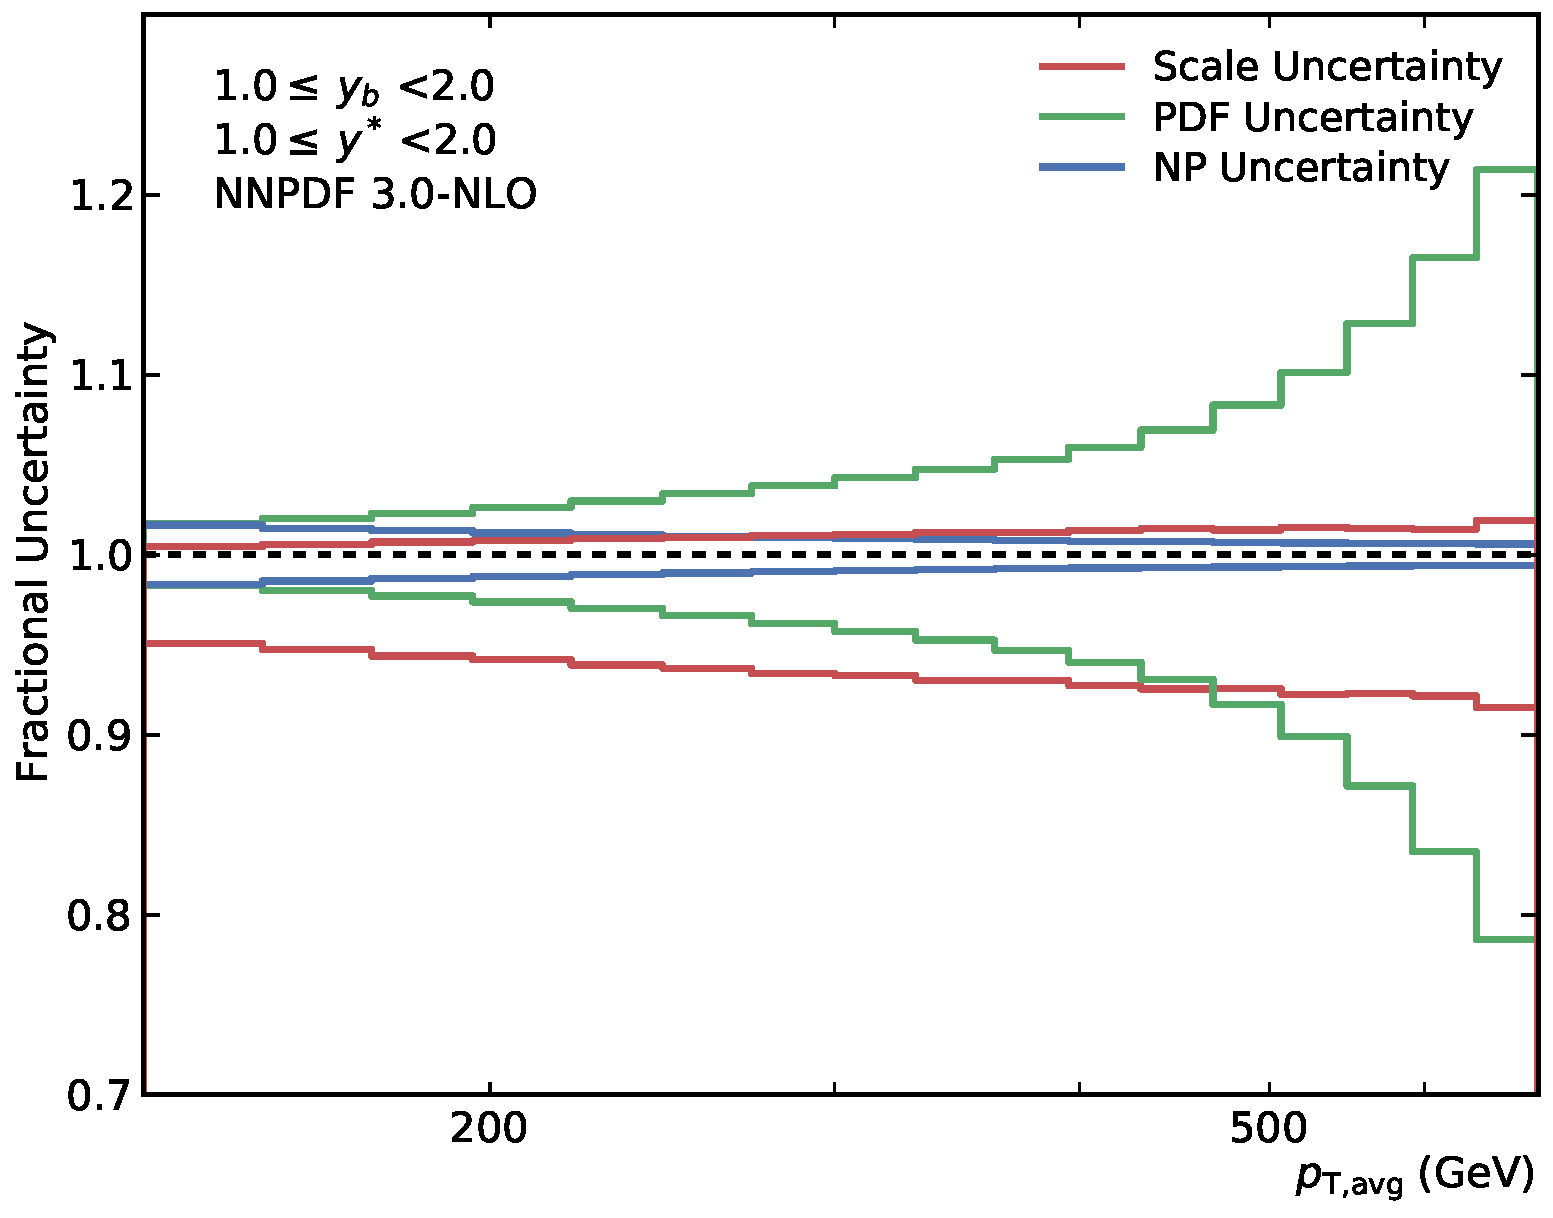
\includegraphics[width=0.45\textwidth]{figures/theory/theo_unc_yb1ys1.pdf}\hfill
    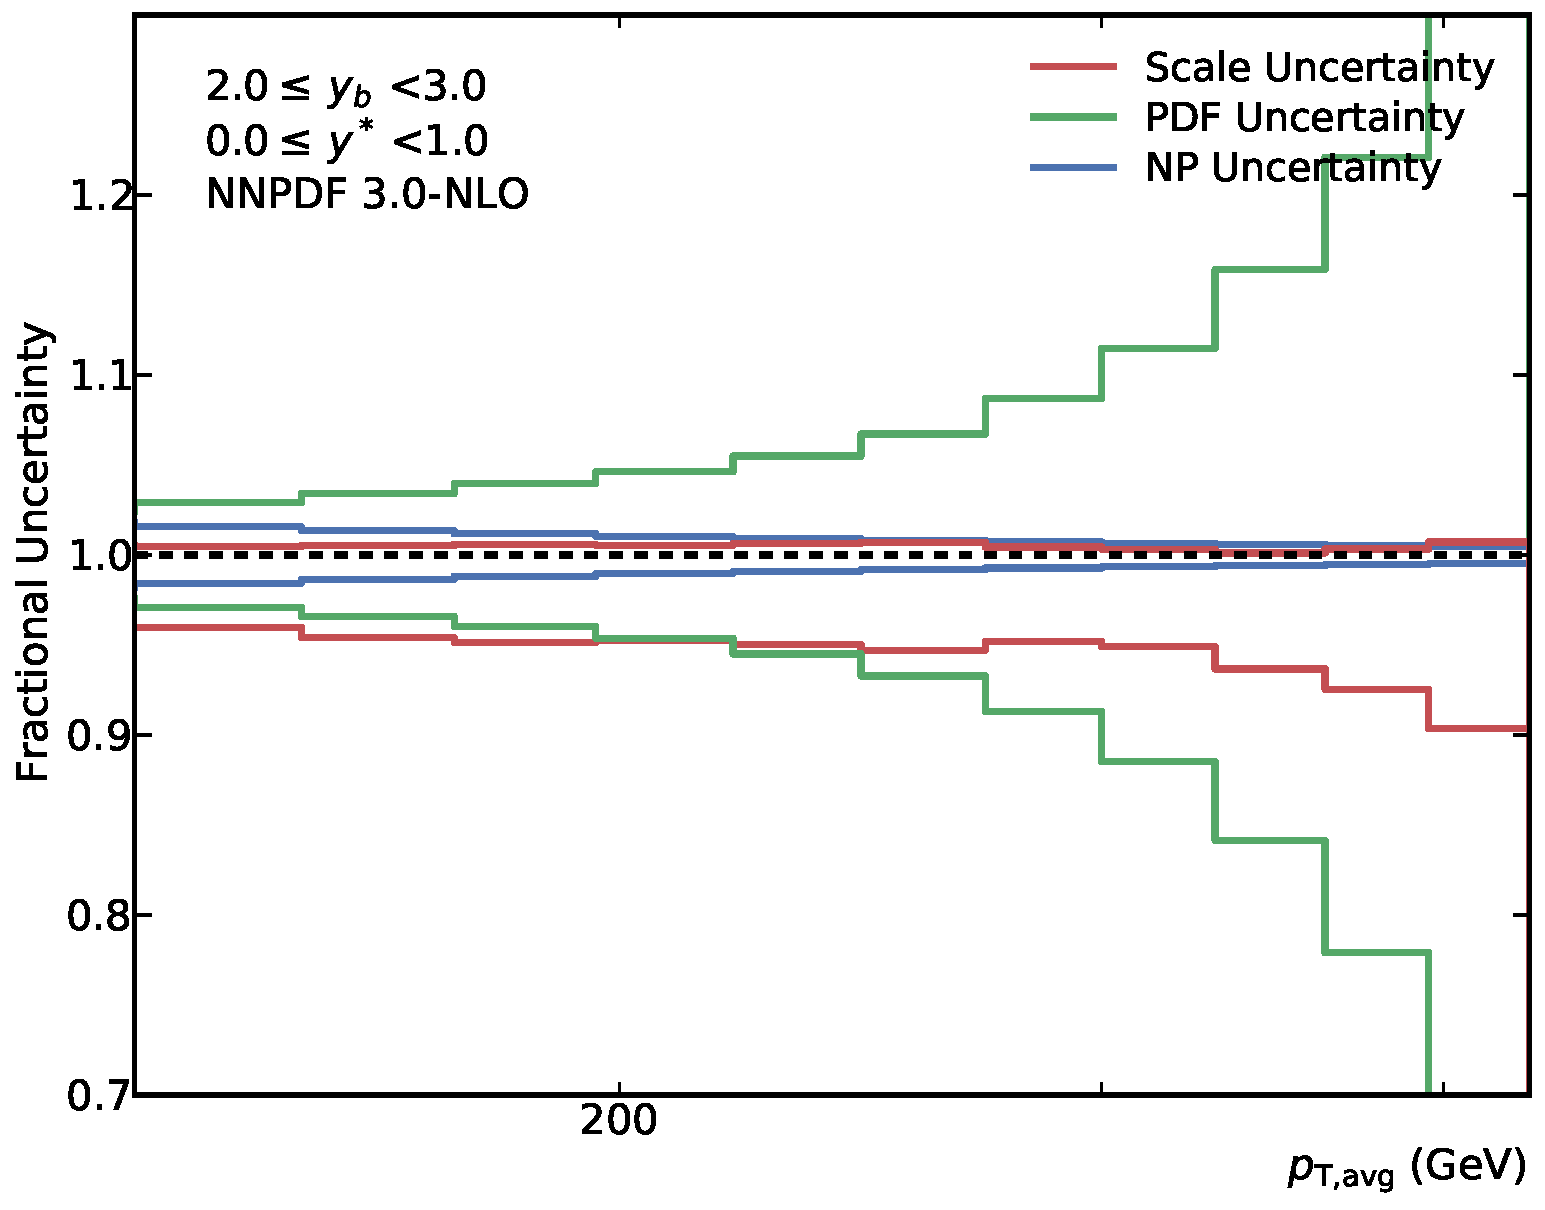
\includegraphics[width=0.45\textwidth]{figures/theory/theo_unc_yb2ys0.pdf}
    \caption{Overview of the theoretical uncertainties of the NLO prediction.
    The scale uncertainty is the dominant uncertainty in the low-\pt region. At
high-\pt and especially in the forward region, the PDF uncertainty becomes
dominant. The NP uncertainty is sizeable only in low-\pt region and becomes
negligible at higher \pt when the NP correction approaches unity.}
    \label{fig:theo_uncertainties}
\end{figure}
